\documentclass{article}
\usepackage{amsmath}
\usepackage{hyperref}
\usepackage{listings}

\title{The name... is speedagean: Improving performance of LTE and NR in ns-3}
\author{Gabriel}
\date{\today}

\begin{document}
\maketitle

\begin{abstract}
\end{abstract}

\section{Ever growing complexity and performance implications}

I haven't blogged in a while. Didn't have the time to do it. During this time,
I left the \href{https://cic.unb.br/}{Universidade de Brasília} and joined
\href{https://www.cttc.cat/}{CTTC}.

One of CTTC clients was concerned with the growing complexity and simulation
runtime, which drastically limit the scalability of simulations, unless you
want to wait a few days for a few seconds worth of a large simulation scenario
to finish.

I have been working on performance optimization since 2010, during my undergrad
thesis/final work, so it is just natural I needed to profile the simulations
and provide some improvements.

The latest feature CTTC has been working on is MIMO, which allows for the
transmission of multiple spatial data streams to increase throughput and
reduce latency. This is done by using a wack ton of antennas in an array, that
are controlled in groups called 'antenna ports'.

Note: I am no specialist in MIMO, so feel free to correct me.

The problem with these many antennas and ports, is that we used to have a single
channel calculation per UE-eNB/gNB pair transmission per subband (resource block),
which was already split into beam clusters. So we already had $O(n^3)$ complexity,
implemented with 3 nested for loops. Now, we need to do these same calculation,
but FOR EACH AND EVERY SENDER/RECEIVER PORT PAIR COMBINATION. This means our
complexity grew to $O(n^5)$.

Note: it is not actually $O(n^5)$, but
$O(nRb\times nReceivers \times nAntennaTx \times nAntennaRx \times nCluster)$,
but I prefer the compact version for simplicity.

And it gets worse, because this is just one of the computations that needs to be done.
MIMO is typically implemented using a codebook to search for the appropriate
precoding matrix, which the UE brute-forces a search to find the indices
of the codebook known as $i_{1}$ and $i_{2}$ for wide-band and sub-band.
This process consumes a lot of power in hardware, which sucks for battery,
but at least it is fast, since the functional units that make the calculations
can be simply copy-pasted to test and compare multiple combinations quickly.

You don't have that luxury when working with software.
So you got to use hardware efficiently.

I'm not going to enter into details on how to profile anything, because
\href{https://www.nsnam.org/docs/manual/html/profiling.html}
{I've have already written an entire section in the ns-3 manual for that}.

Just let's review the basics on graphical analysis (this isn't real science, but whatever...).

Below we have Figure \ref{fig:profiling-basics}, showing how the profiling of a program looks
like. In the vertical axis, we have the program stack, which gets sampled by the profiler
every few milliseconds or whatever frequency you configure it to sample.

In the horizontal axis you have 100\% of total CPU time. This is important, because
optimizations are not going to reduce the size of these bars, just the size of the
bar of the piece of code that was optimized. The rest of the code will have their bars
widened, to show they are now more significant.

\begin{figure}
    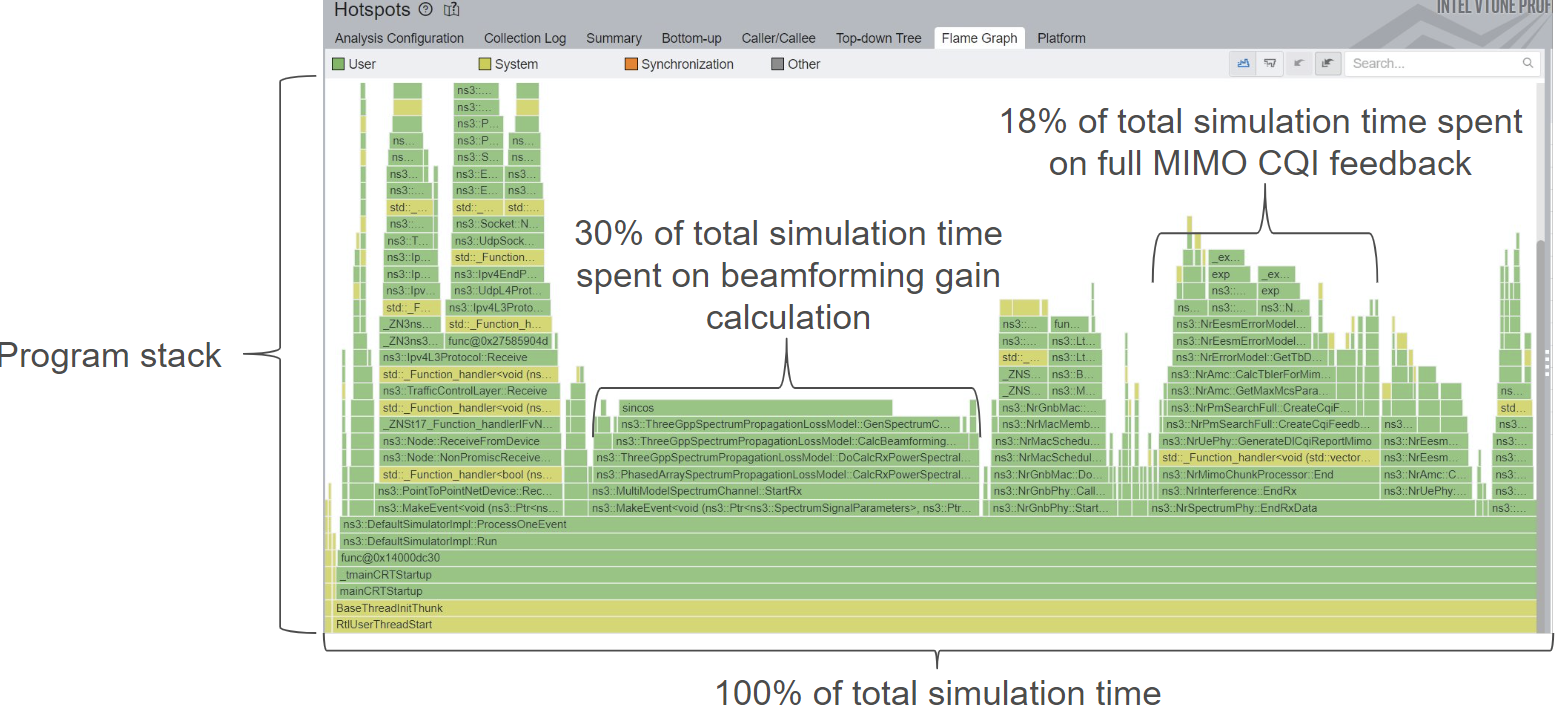
\includegraphics[width=1.0\textwidth,height=1.0\textheight]{"/assets/img/2024-03-07-the-name-is-the-speedagean/profiling-basics.png"}
    \caption{Performance profiling of cttc-nr-mimo-demo with MIMO feedback, of release nr-3.0.y}
    \label{fig:profiling-basics}
\end{figure}

With this introduction, let's proceed to some profiling results and optimizations for
their primary bottlenecks.

\section{Default cttc-nr-mimo-demo settings with MIMO feedback}

This scenario is pretty vanilla, with small number of antennas, antenna ports,
just a single UE and gNB, in a static scenario. First, let's take a look at
the initial profiling results. This was taken with nr-3.0 and ns-3.41 releases.
Following profiles are cumulative, getting speedups from the previous optimizations.

\subsection{Delay computation in ThreeGppSpectrumPropagationLossModel}

You can see in Figure \ref{fig:cache-sincos-before} that a huge fraction of the
total simulation time was spent on ThreeGppSpectrumPropagationLossModel::CalcBeamformingGain,
and most of it is calculating sincos.

\begin{figure}
    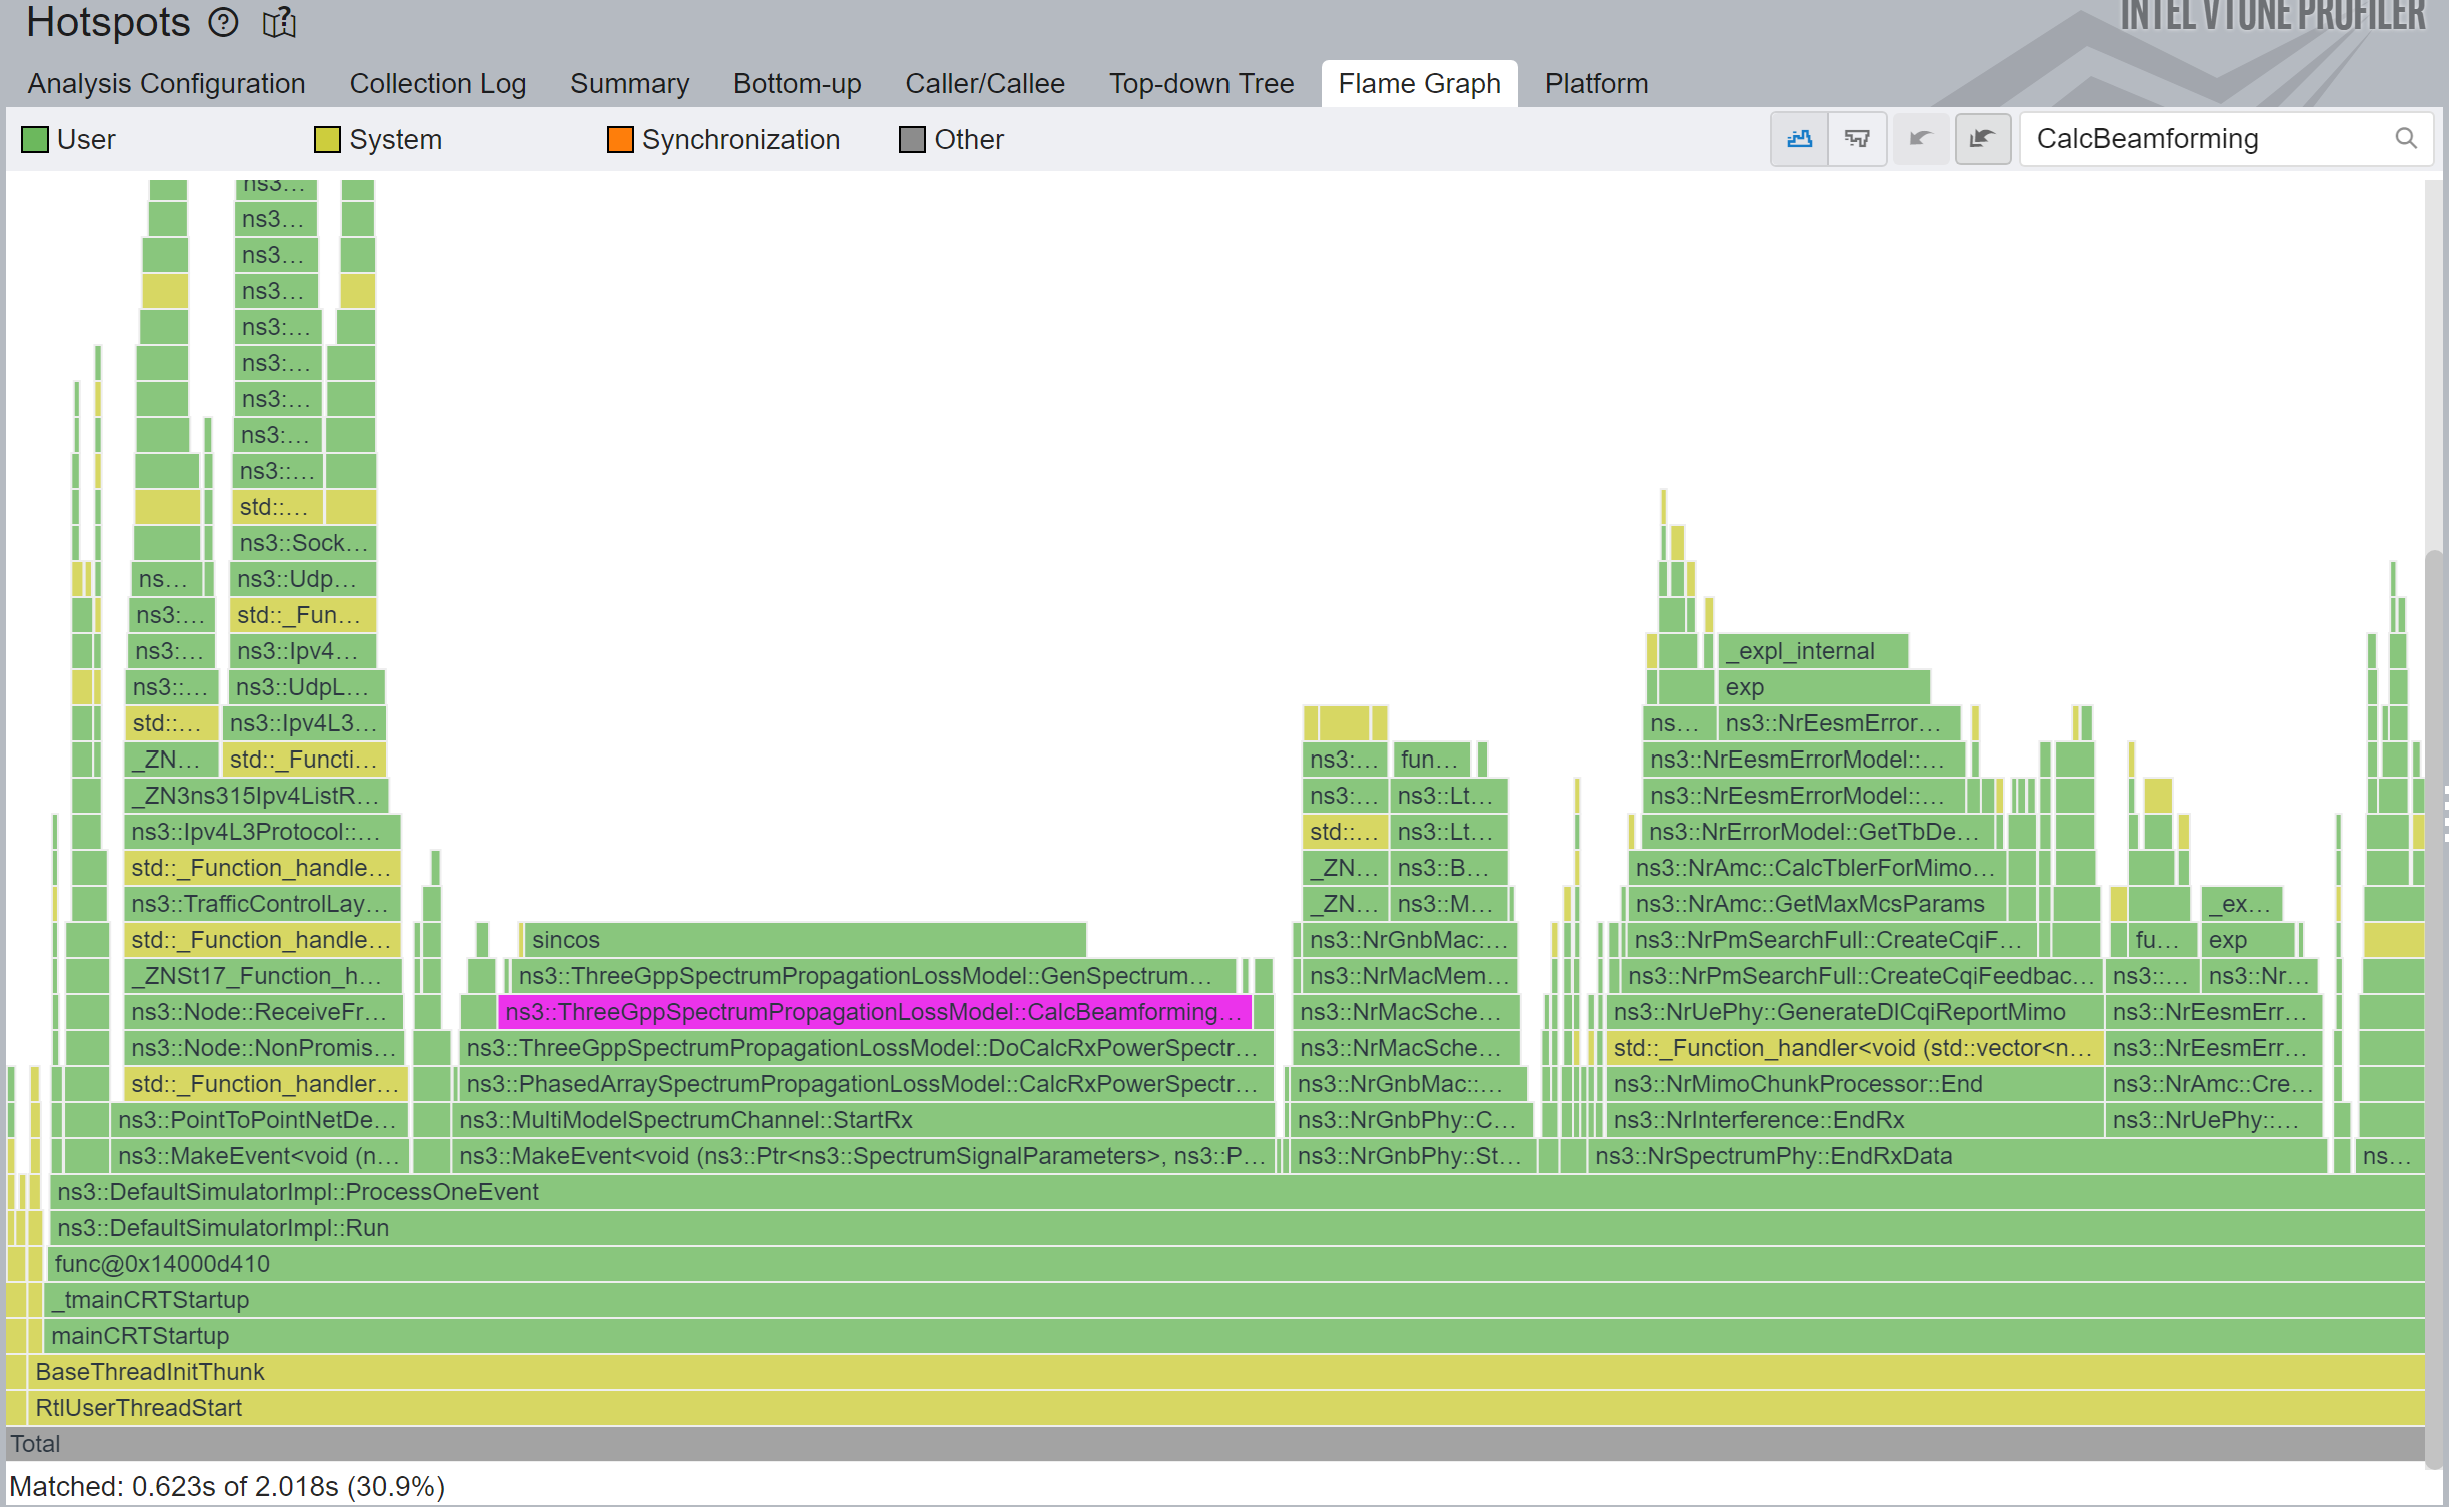
\includegraphics[width=1.0\textwidth,height=1.0\textheight]{"/assets/img/2024-03-07-the-name-is-the-speedagean/cache-sincos-before.png"}
    \caption{Before optimization}
    \label{fig:cache-sincos-before}
\end{figure}

This sincos means we are computing both a sin and a cosine of the same angle together,
which is more efficient than separately.

The respective piece of code that calls these many sincos is the following loop:

\begin{lstlisting}
 while (vit != inPsd->ValuesEnd())
    {
        if ((*vit) != 0.00)
        {
            double fsb = (*sbit).fc; // center frequency of the sub-band
            for (auto rxPortIdx = 0; rxPortIdx < numRxPorts; rxPortIdx++)
            {
                for (auto txPortIdx = 0; txPortIdx < numTxPorts; txPortIdx++)
                {
                    std::complex<double> subsbandGain(0.0, 0.0);

                    for (size_t cIndex = 0; cIndex < numCluster; cIndex++)
                    {
                        double delay = -2 * M_PI * fsb * (channelParams->m_delay[cIndex]);
                        subsbandGain += directionalLongTerm(rxPortIdx, txPortIdx, cIndex) *
                                        doppler[cIndex] *
                                        std::complex<double>(cos(delay), sin(delay)); // <<<< HERE
                    }
                    // Multiply with the square root of the input PSD so that the norm (absolute
                    // value squared) of chanSpct will be the output PSD
                    chanSpct->Elem(rxPortIdx, txPortIdx, iRb) = sqrt(*vit) * subsbandGain;
                }
            }
        }
        vit++;
        sbit++;
        iRb++;
    }
\end{lstlisting}

To save up in so many sincos, I've tried a bunch of different techniques:
memoization, lookup tables, cordic, fast sincos implementations, but none
gave great results.

And the reason is simple: this is the $O(n^5)$ loop I mentioned before.
You can't see the loop above it, so it is technically $O(n^4)$, but this
our archnemesis.

If we want to scale, we need to get this sincos out of here in some way.
After carefully inspecting where exactly we get the \emph{m\_delay}, I noticed
these values are not always updated, so there is no need for us to recompute
them every single time. Also, they do not even depend in the number of ports,
so it is criminally expensive to put them inside of these loops. You would
hope the compiler to optimize that, but you don't get these kind of
optimization while debugging.

What I ended up doing was to cache these delay calculation until channel
conditions change. These were merged in
\href{https://gitlab.com/nsnam/ns-3-dev/-/merge_requests/1427}{ns-3-dev MR1427}.

The caching section is the following:

\begin{lstlisting}
// Precompute the delay until numRb, numCluster or RB width changes
    // Whenever the channelParams is updated, the number of numRbs, numClusters
    // and RB width (12*SCS) are reset, ensuring these values are updated too
    double rbWidth = inPsd->ConstBandsBegin()->fh - inPsd->ConstBandsBegin()->fl;

    if (channelParams->m_cachedDelaySincos.GetNumRows() != numRb ||
        channelParams->m_cachedDelaySincos.GetNumCols() != numCluster ||
        channelParams->m_cachedRbWidth != rbWidth)
    {
        channelParams->m_cachedRbWidth = rbWidth;
        channelParams->m_cachedDelaySincos = ComplexMatrixArray(numRb, numCluster);
        auto sbit = inPsd->ConstBandsBegin(); // band iterator
        for (unsigned i = 0; i < numRb; i++)
        {
            double fsb = (*sbit).fc; // center frequency of the sub-band
            for (std::size_t cIndex = 0; cIndex < numCluster; cIndex++)
            {
                double delay = -2 * M_PI * fsb * (channelParams->m_delay[cIndex]);
                channelParams->m_cachedDelaySincos(i, cIndex) =
                    std::complex<double>(cos(delay), sin(delay));
            }
            sbit++;
        }
    }
\end{lstlisting}

And now we just read the values from \emph{channelParams\rightarrow m\_cachedDelaySincos}.
in the loop shown before.

The results are perplexing, in my humble opinion: 1.36x speedup in total simulation time,
and 11x speedup in that specific function, as shown in Figure \ref{fig:cache-sincos-after}.
\begin{figure}
    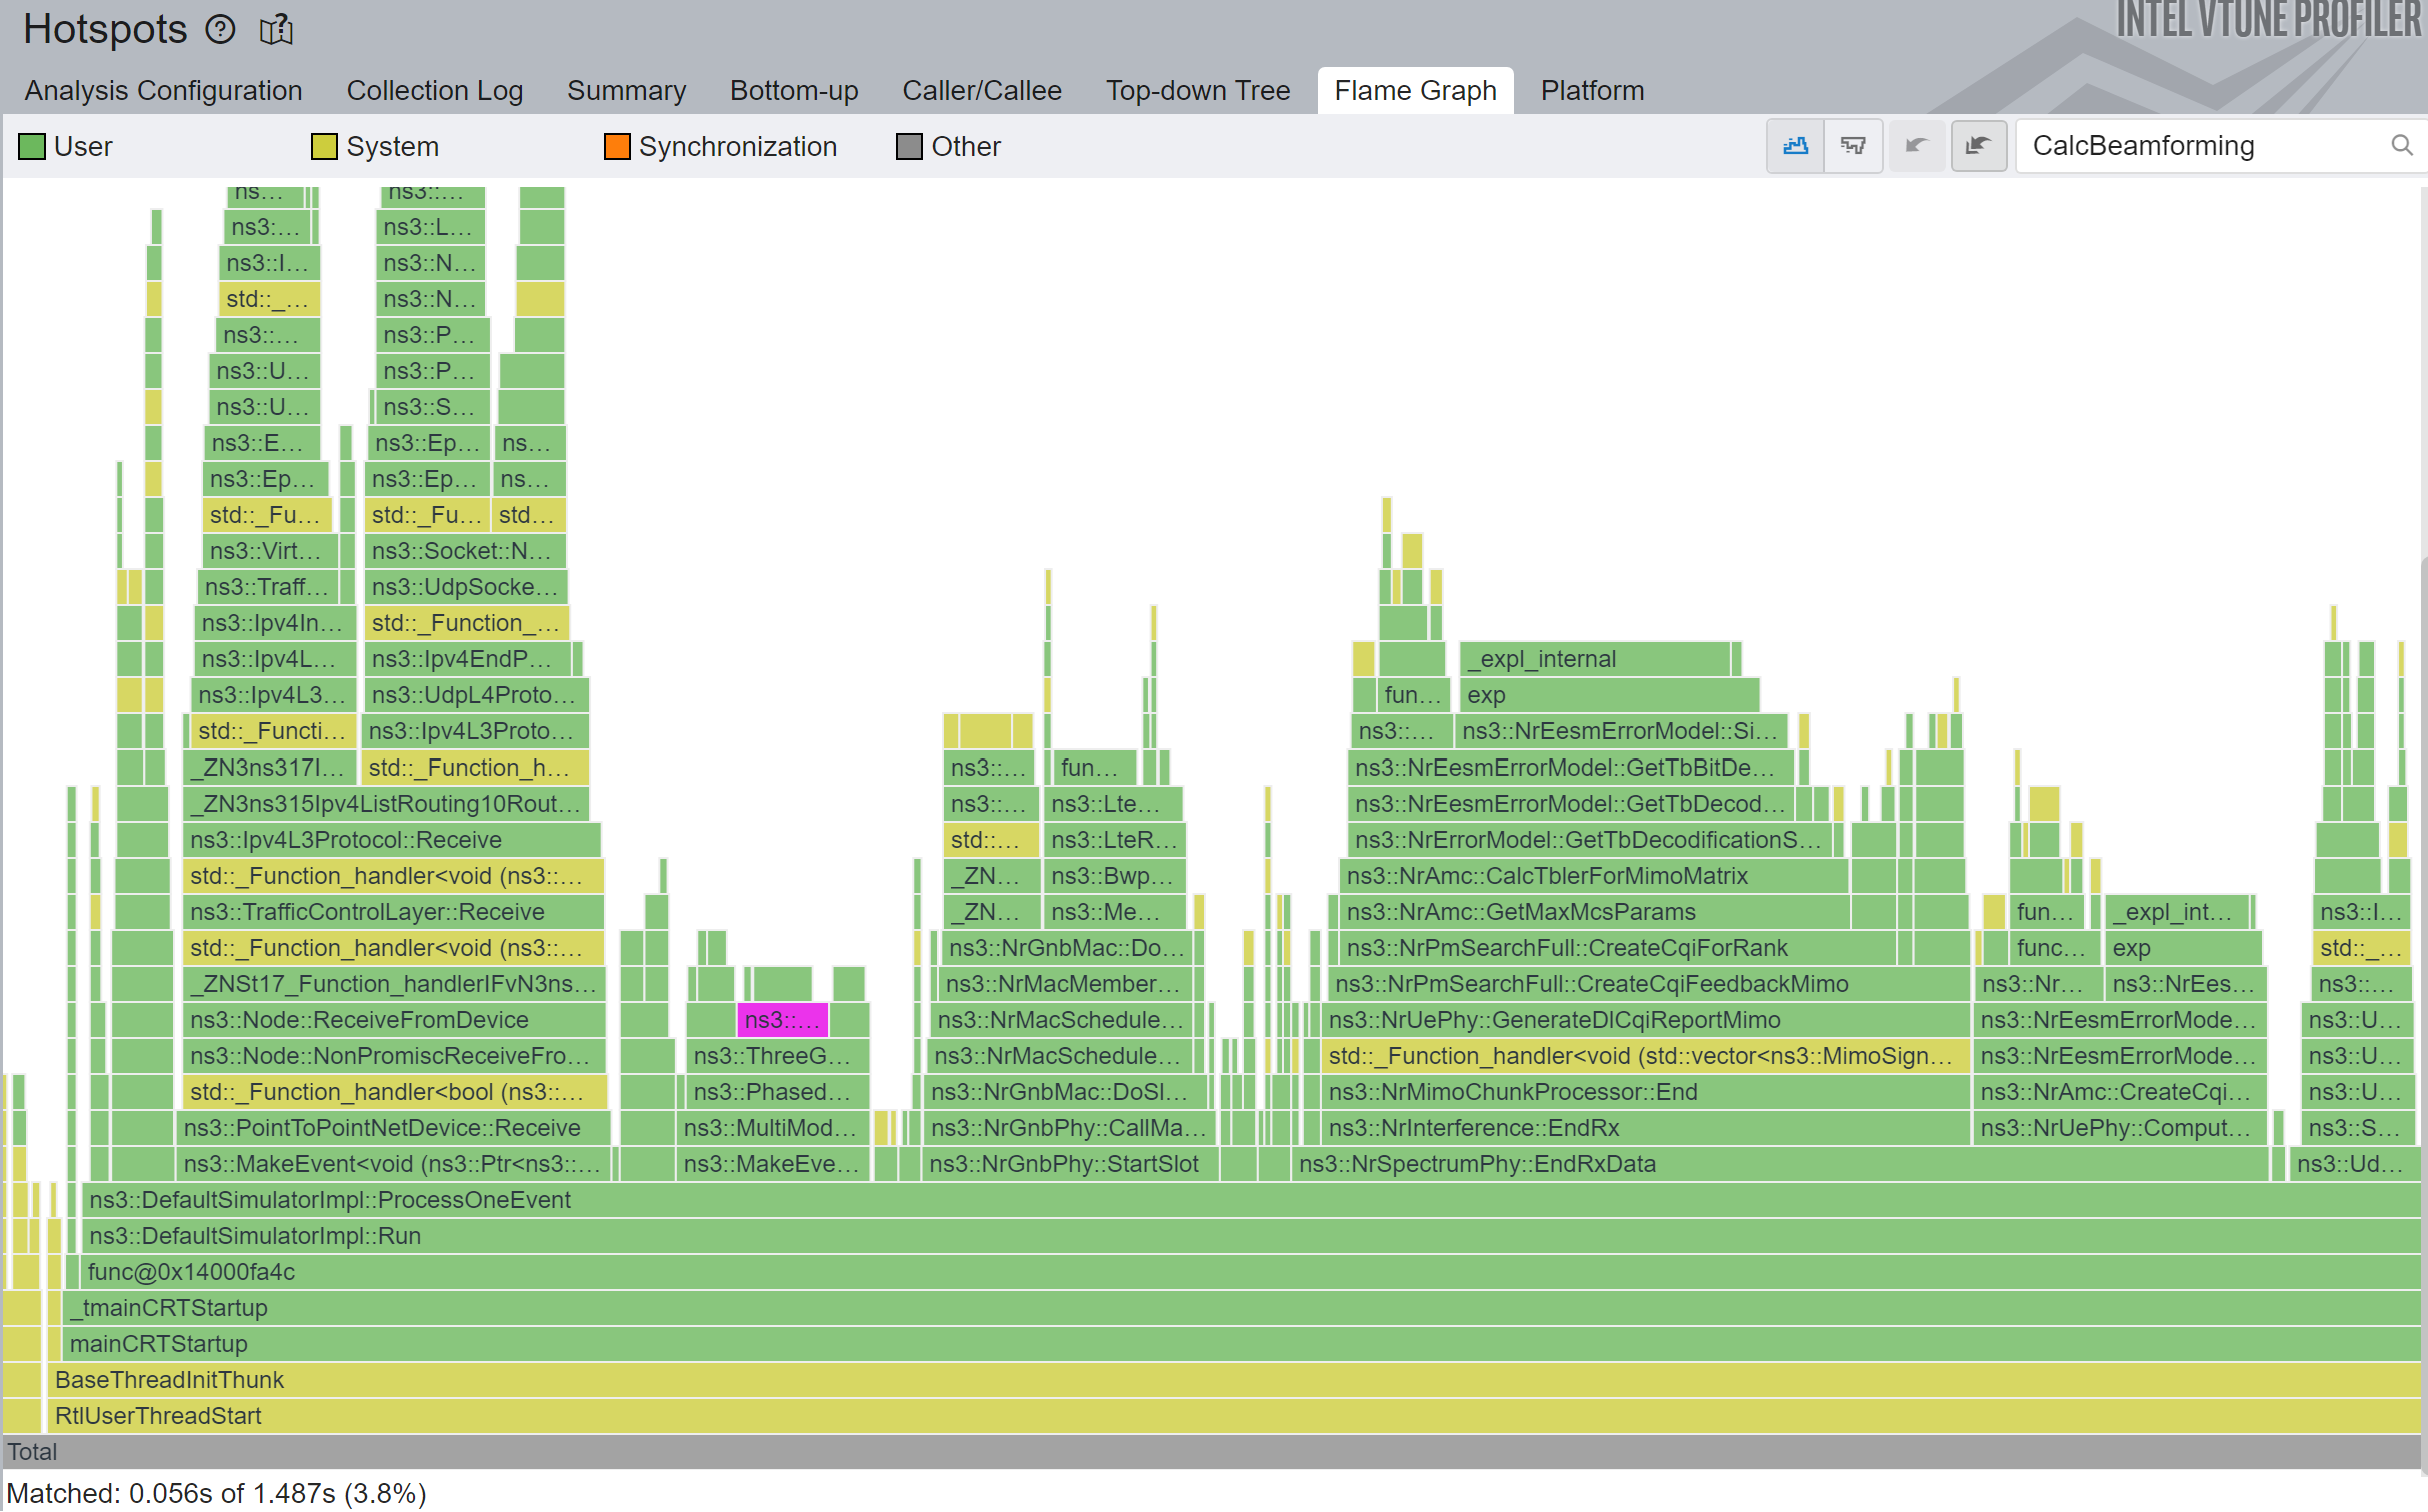
\includegraphics[width=1.0\textwidth,height=1.0\textheight]{"/assets/img/2024-03-07-the-name-is-the-speedagean/cache-sincos-after.png"}
    \caption{After optimization}
    \label{fig:cache-sincos-after}
\end{figure}

We are in for a great start.

\subsection{Exponential SINR in NrEesmErrorModel}

If you look at the profiling results from the previous section, you are
going to notice the largest column is now an \emph{exp} function call.

This \emph{exp} is called in the following function:

\begin{lstlisting}
double
NrEesmErrorModel::SinrExp(const SpectrumValue& sinr, const std::vector<int>& map, uint8_t mcs) const
{
    // it returns sum_n (exp (-SINR/beta))
    NS_LOG_FUNCTION(sinr << &map << (uint8_t)mcs);
    NS_ABORT_MSG_IF(map.empty(),
                    " Error: number of allocated RBs cannot be 0 - EESM method - SinrEff function");

    double SINRexp = 0.0;
    double SINRsum = 0.0;
    double beta = GetBetaTable()->at(mcs);
    for (int i : map)
    {
        double sinrLin = sinr[i];
        SINRexp = exp(-sinrLin / beta);
        SINRsum += SINRexp;
    }
    return SINRsum;
}
\end{lstlisting}

There isn't anything crazy about this function, other than the slow \emph{exp}
math function. In the Figure \ref{fig:sinr-exp-before} below we can see the
profiling results before the proposed optimizations.

\begin{figure}
    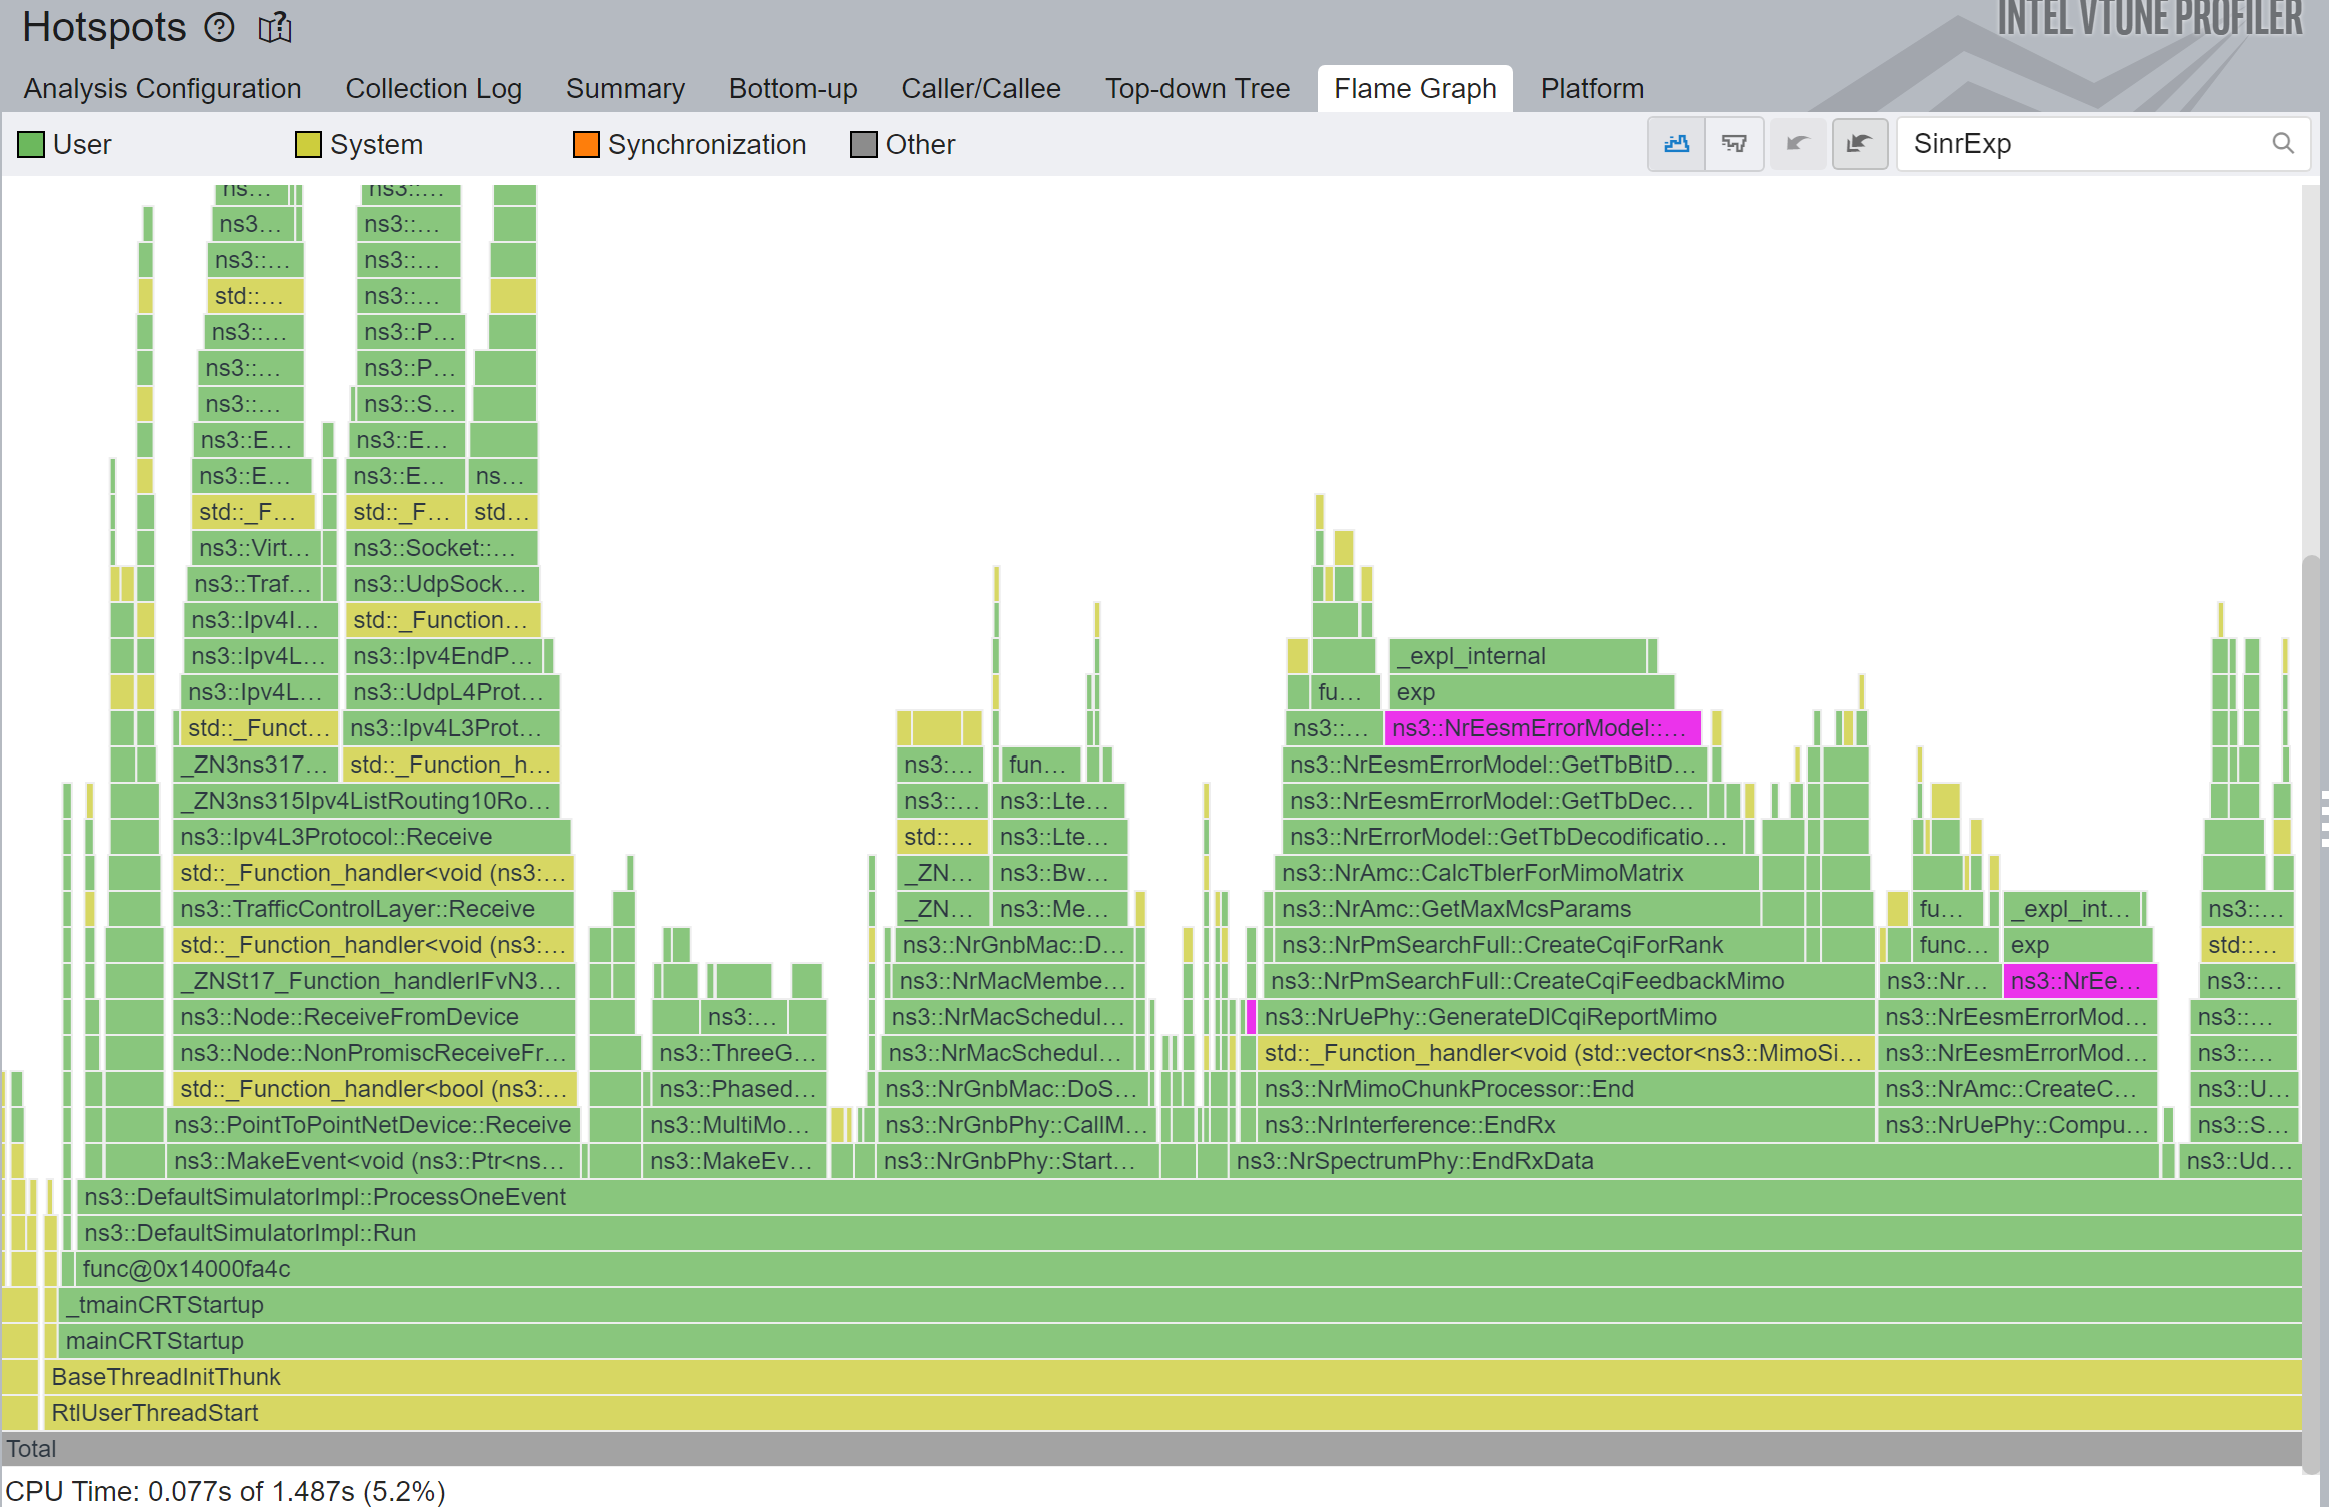
\includegraphics[width=1.0\textwidth,height=1.0\textheight]{"/assets/img/2024-03-07-the-name-is-the-speedagean/sinr-exp-before.png"}
    \caption{Before optimization}
    \label{fig:sinr-exp-before}
\end{figure}

But it turns out there are plenty of brilliant mathematicians working tirelessly
to produce fast approximations for these math primitives. I found one of these
approximations in "Simple multiple precision algorithms for exponential functions",
by Leonid Moroz, Volodymyr Samotyy, Zbigniew Kokosiński and Paweł Gepner, published in
the \href{https://ieeexplore.ieee.org/document/9810030}{IEEE Signal Processing Magazine 39(4):130 - 137 (2022)}.

Their solution works brilliantly and is a lot faster than the default glibc exponential.
I am very grateful that they accepted to license their code under the very permissive MIT license.

Their implementation for floats look like this:

\begin{lstlisting}
inline float
exp21f(float x)
{
    int z = x * 0x00b8aa3b + 0x3f800000;

    union {
        int i;
        float f;
    } zii;

    zii.i = z & 0x7f800000;
    int zif = z & 0x007fffff;
    float d1 = 0.40196114e-7f;
    float d2 = 0xf94ee7 + zif;
    float d3 = 0x560e + zif;
    d2 = d1 * d2;
    zif = d2 * d3;
    zii.i |= zif;
    float y = zii.f;
    return y;
}
\end{lstlisting}

After replacing the original code with this one, plus a few additional guards,
we get the following results in Figure \ref{fig:sinr-exp-after}:

\begin{figure}
    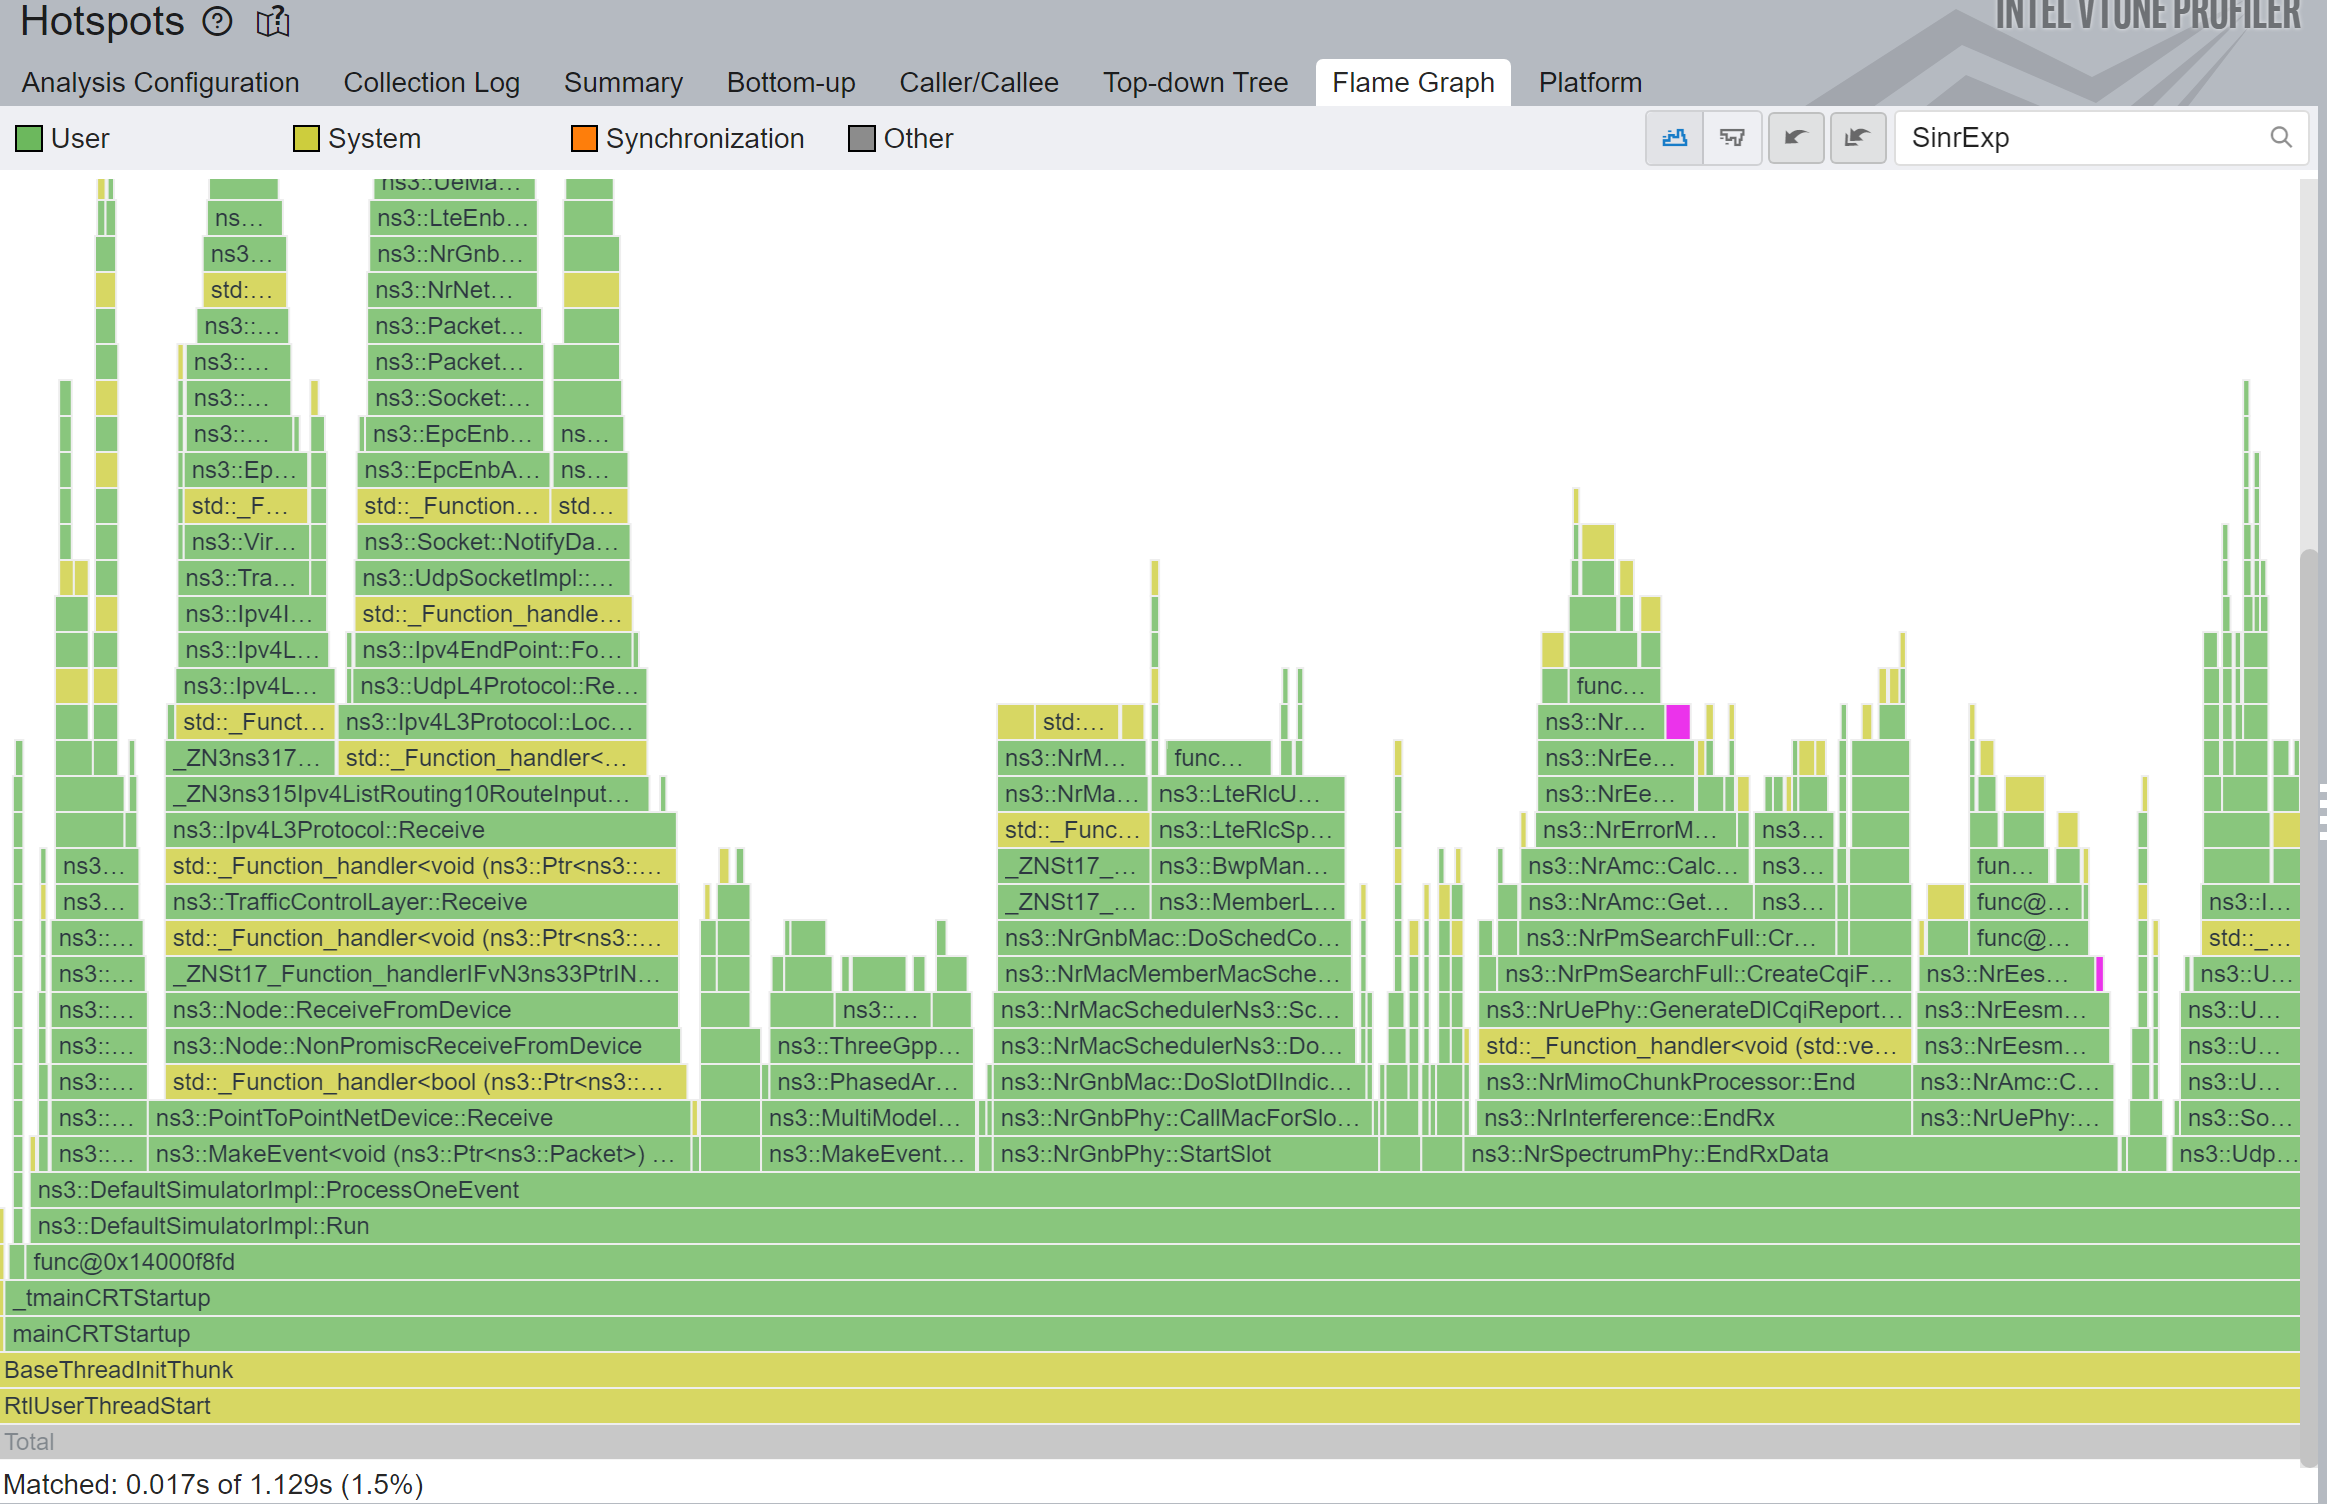
\includegraphics[width=1.0\textwidth,height=1.0\textheight]{"/assets/img/2024-03-07-the-name-is-the-speedagean/sinr-exp-after.png"}
    \caption{After optimization}
    \label{fig:sinr-exp-after}
\end{figure}

Fantastic 1.32x total simulation speedup, and 4.5x speedup in that particular function.

I was very concerned about this patch though, because it is a key value
used to determine the Block-Level Error Rate (BLER) and eventually the
Modulation and Coding Scheme (MCS), which can make
or break the system. In fact, when I tested a different fast implementation,
simulations broke due to the loss of precision, but this implementation
provides enough precision for our use case. An example of that is shown
in the Figure \ref{fig:sinr-exp-prec} below:

\begin{figure}
    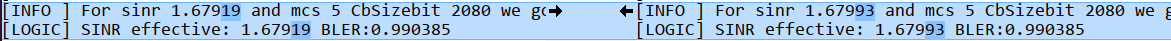
\includegraphics[width=1.0\textwidth,height=1.0\textheight]{"/assets/img/2024-03-07-the-name-is-the-speedagean/sinr-exp-prec.png"}
    \caption{Comparison between precision of custom Exp() function}
    \label{fig:sinr-exp-prec}
\end{figure}

Which means we are good in most cases, but we are still testing it,
in case we missed some important case in our automated test suites.
This patch is currently available as the
\href{https://gitlab.com/cttc-lena/nr/-/merge_requests/111}{nr MR111}.

So far, so good. To the next bottleneck.

\subsection{Keep traces file open throughout the simulation}

This one isn't anything new. I've repeated that time and time again.
In fact I fixed the same issue in LTE, in
\href{https://gitlab.com/nsnam/ns-3-dev/-/merge_requests/814}{ns-3 MR814}.

Opening and closing files during the simulation can be incredibly slow
in slow filesystems (e.g. HDD, network mounts such as the one used by
Windows WSL, Windows due to garbage that is Windows defender).

The code for this was already merged upstream in
\href{https://gitlab.com/cttc-lena/nr/-/merge_requests/113}{nr MR113}.

Below are the Before \ref{fig:keep-traces-open-before},
and After \ref{fig:keep-traces-open-after} figures,
showing the 1.16x total simulation speedup,
or 18x speedup for that particular function.

\begin{figure}
    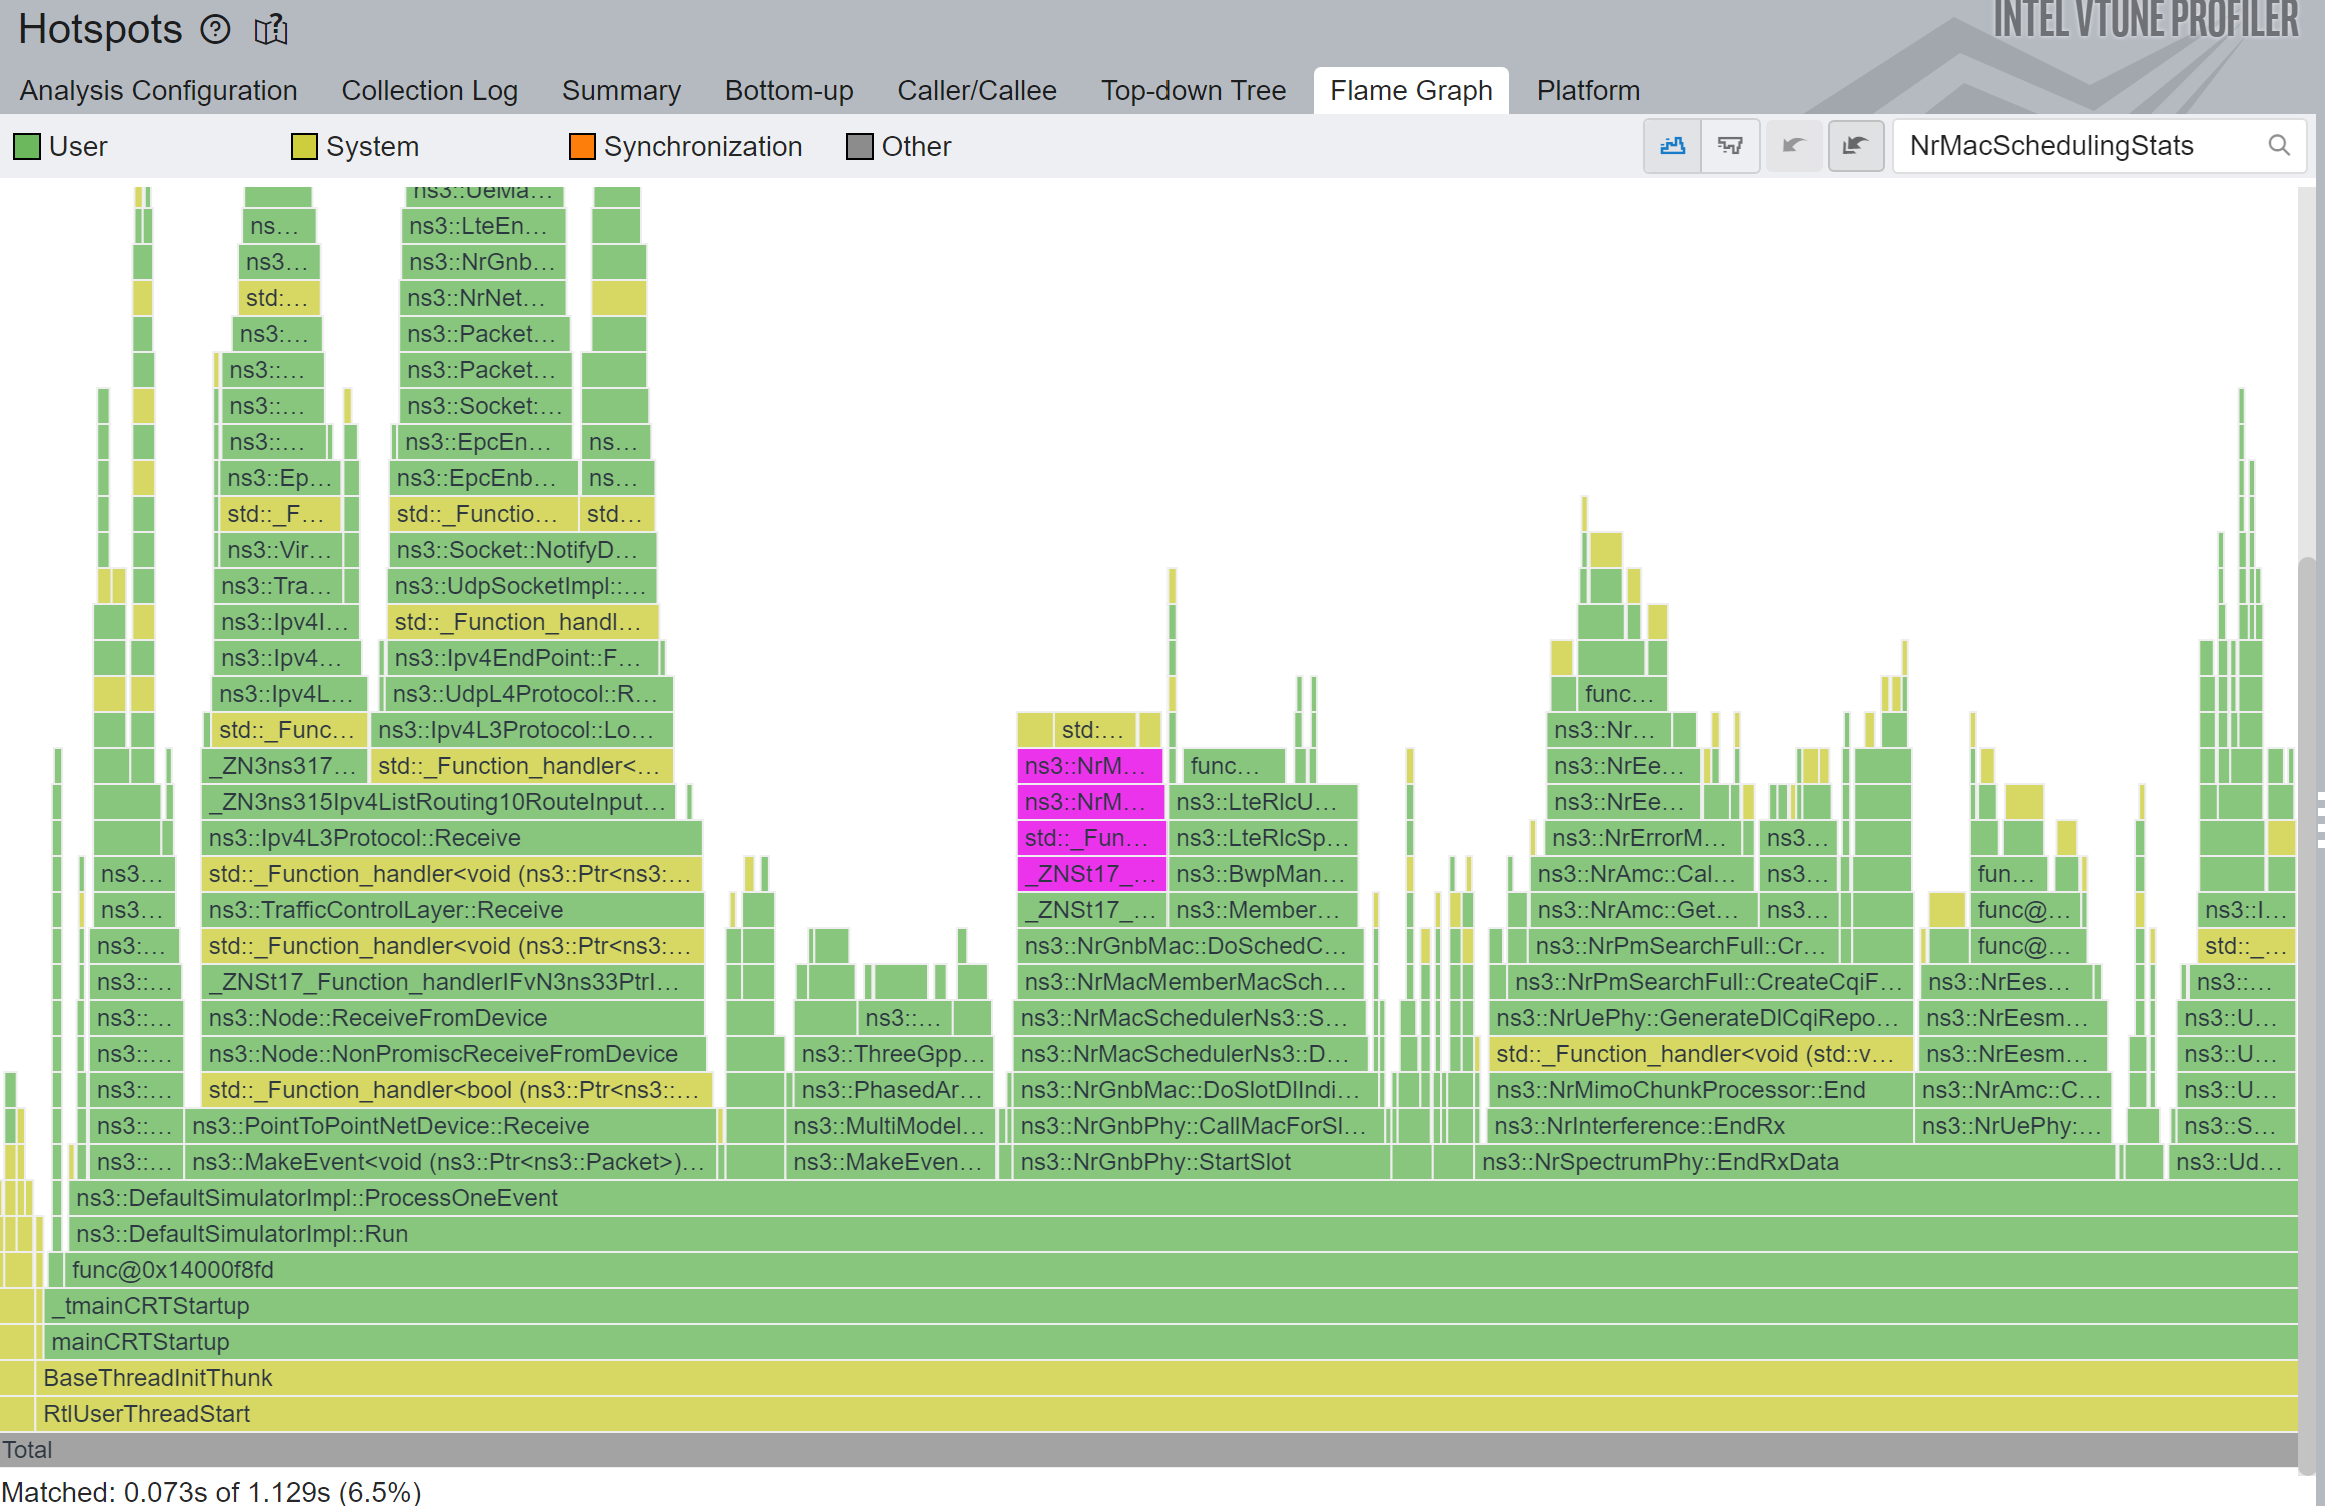
\includegraphics[width=1.0\textwidth,height=1.0\textheight]{"/assets/img/2024-03-07-the-name-is-the-speedagean/keep-traces-open-before.png"}
    \caption{Before optimization}
    \label{fig:keep-traces-open-before}
\end{figure}

\begin{figure}
    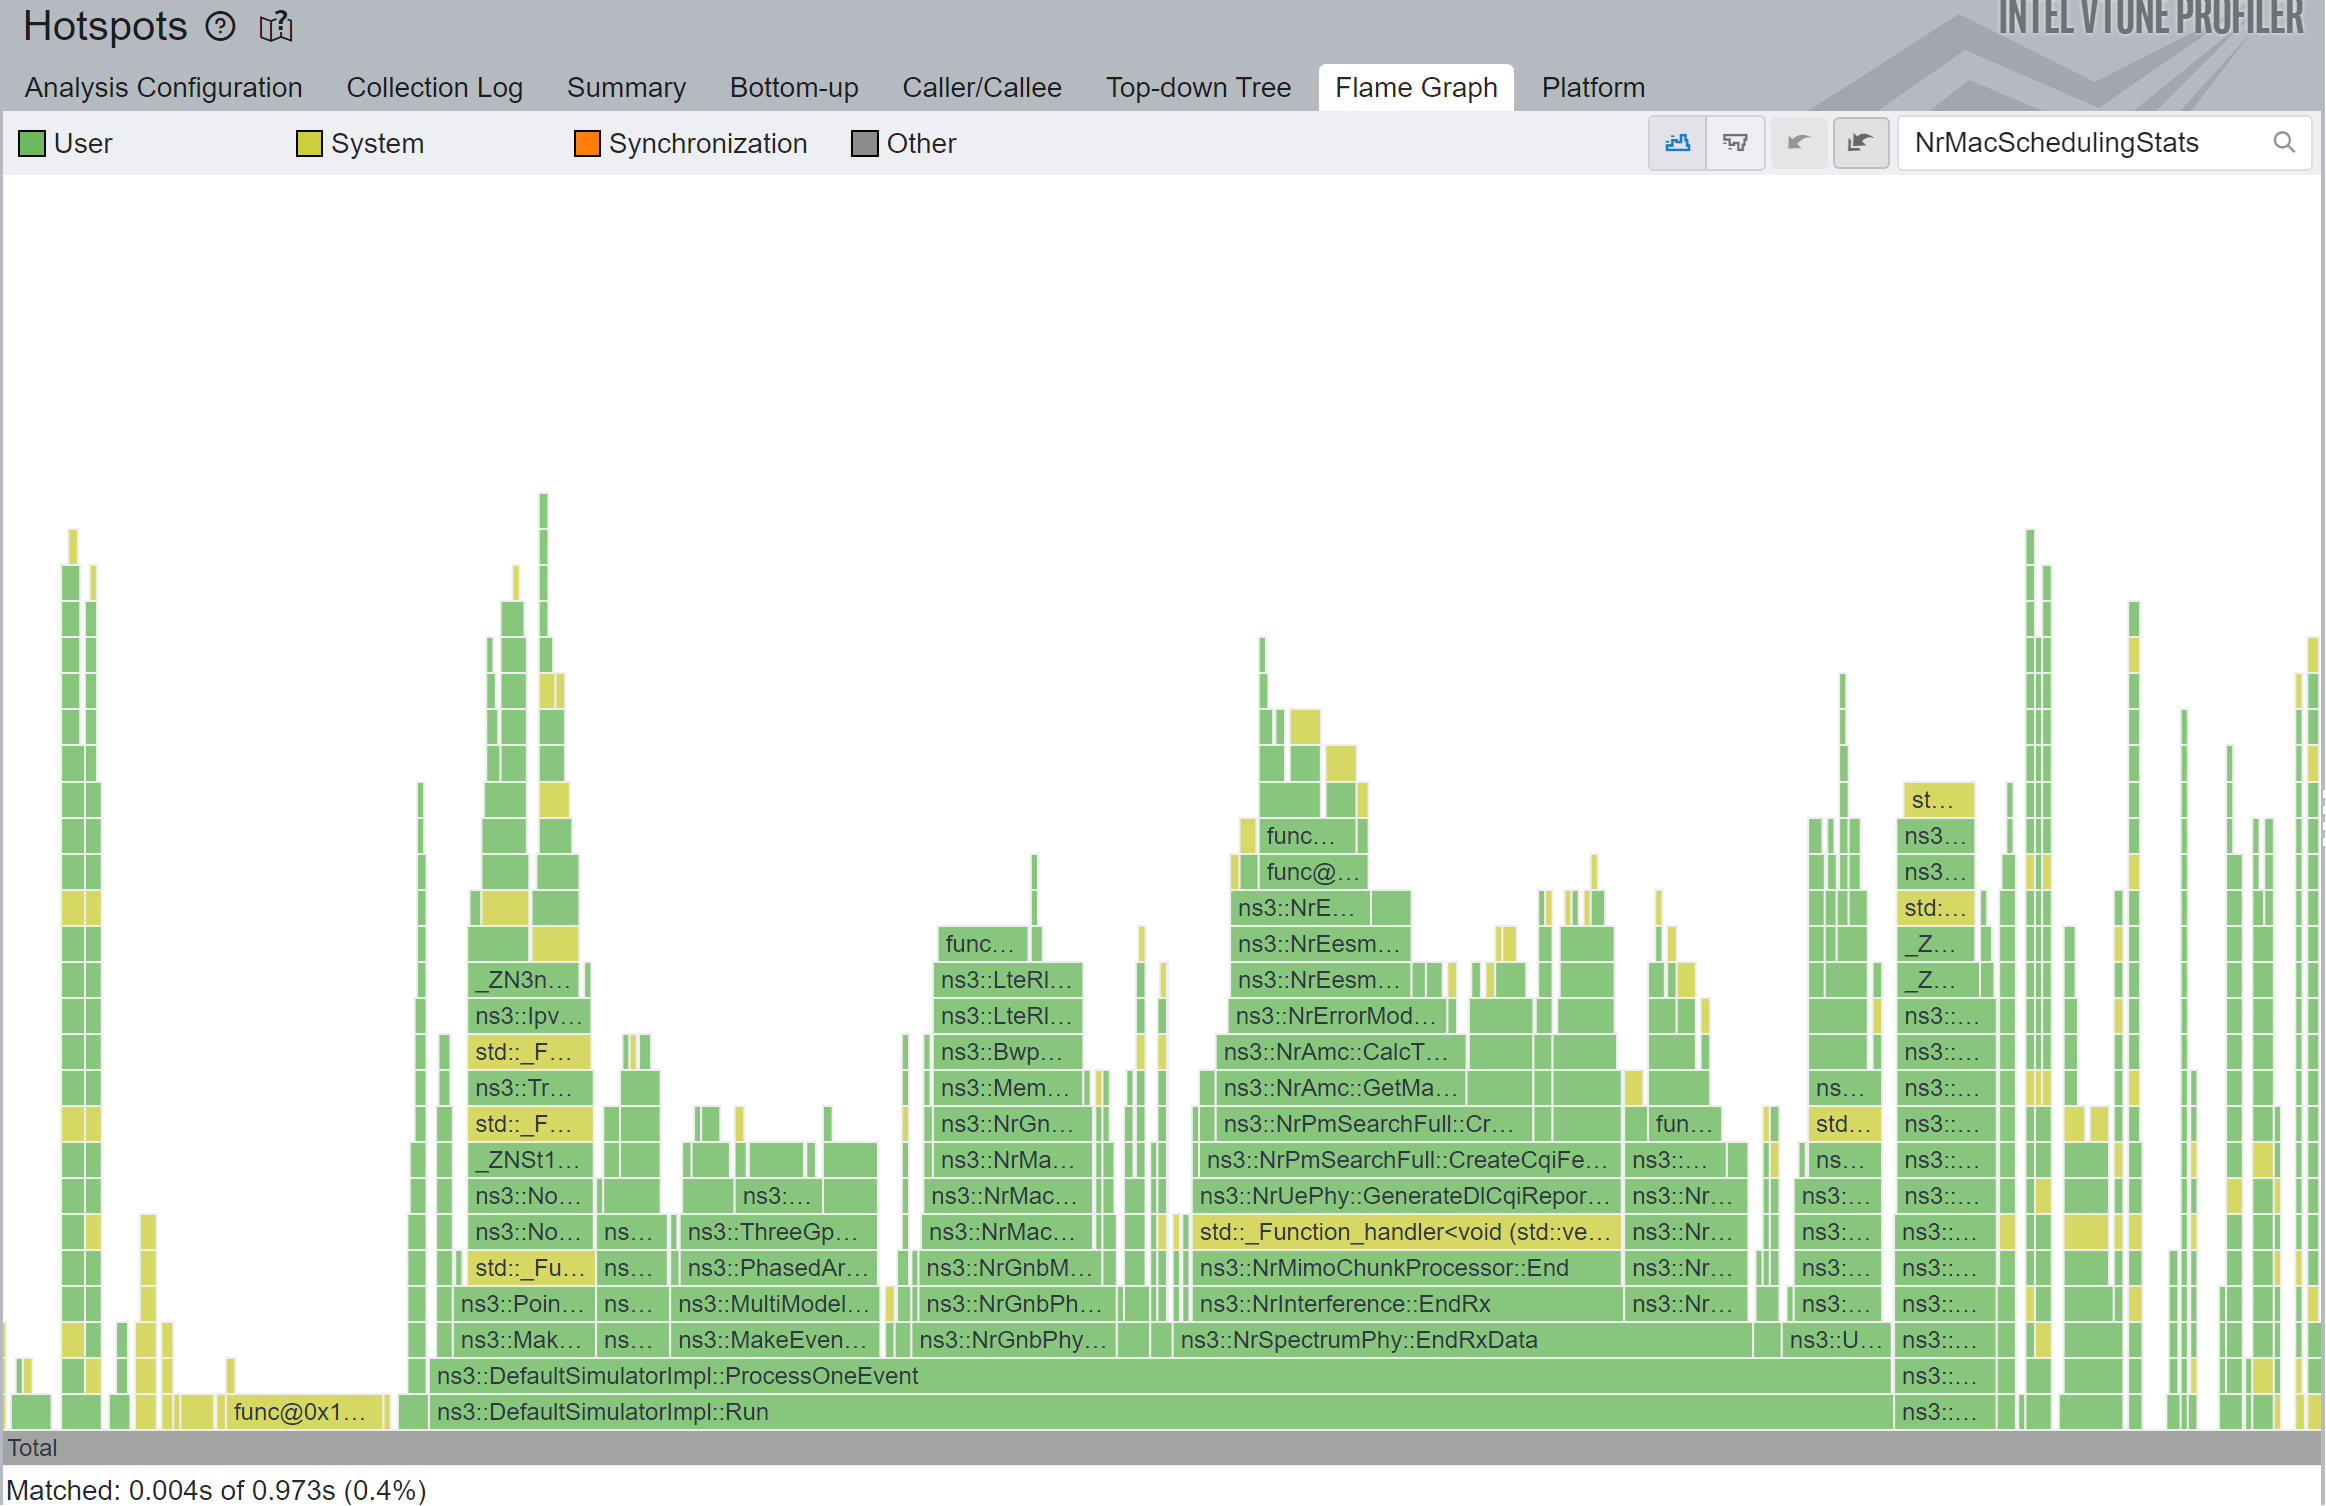
\includegraphics[width=1.0\textwidth,height=1.0\textheight]{"/assets/img/2024-03-07-the-name-is-the-speedagean/keep-traces-open-after.png"}
    \caption{After optimization}
    \label{fig:keep-traces-open-after}
\end{figure}

\subsection{Prevent unnecessary copy}

C++ kind of sucks in being explicit about deep copies.
In fact, it is very easy to deep copy a huge structure
and pay a hefty price for a single missing \emph{&} character.

And that happened in the following code of nr:

\begin{lstlisting}
double
NrEesmErrorModel::MappingSinrBler(double sinr, uint8_t mcs, uint32_t cbSizeBit)
{
...
    const auto cbMap = GetSimulatedBlerFromSINR()->at(bg_type).at(mcs); // <<<< HERE
    auto cbIt = cbMap.upper_bound(cbSizeBit);
...
\end{lstlisting}

Adding the missing \emph{&} resulted in a 1.15x total simulation speedup,
or 18x speedup in that particular function.

\begin{figure}
    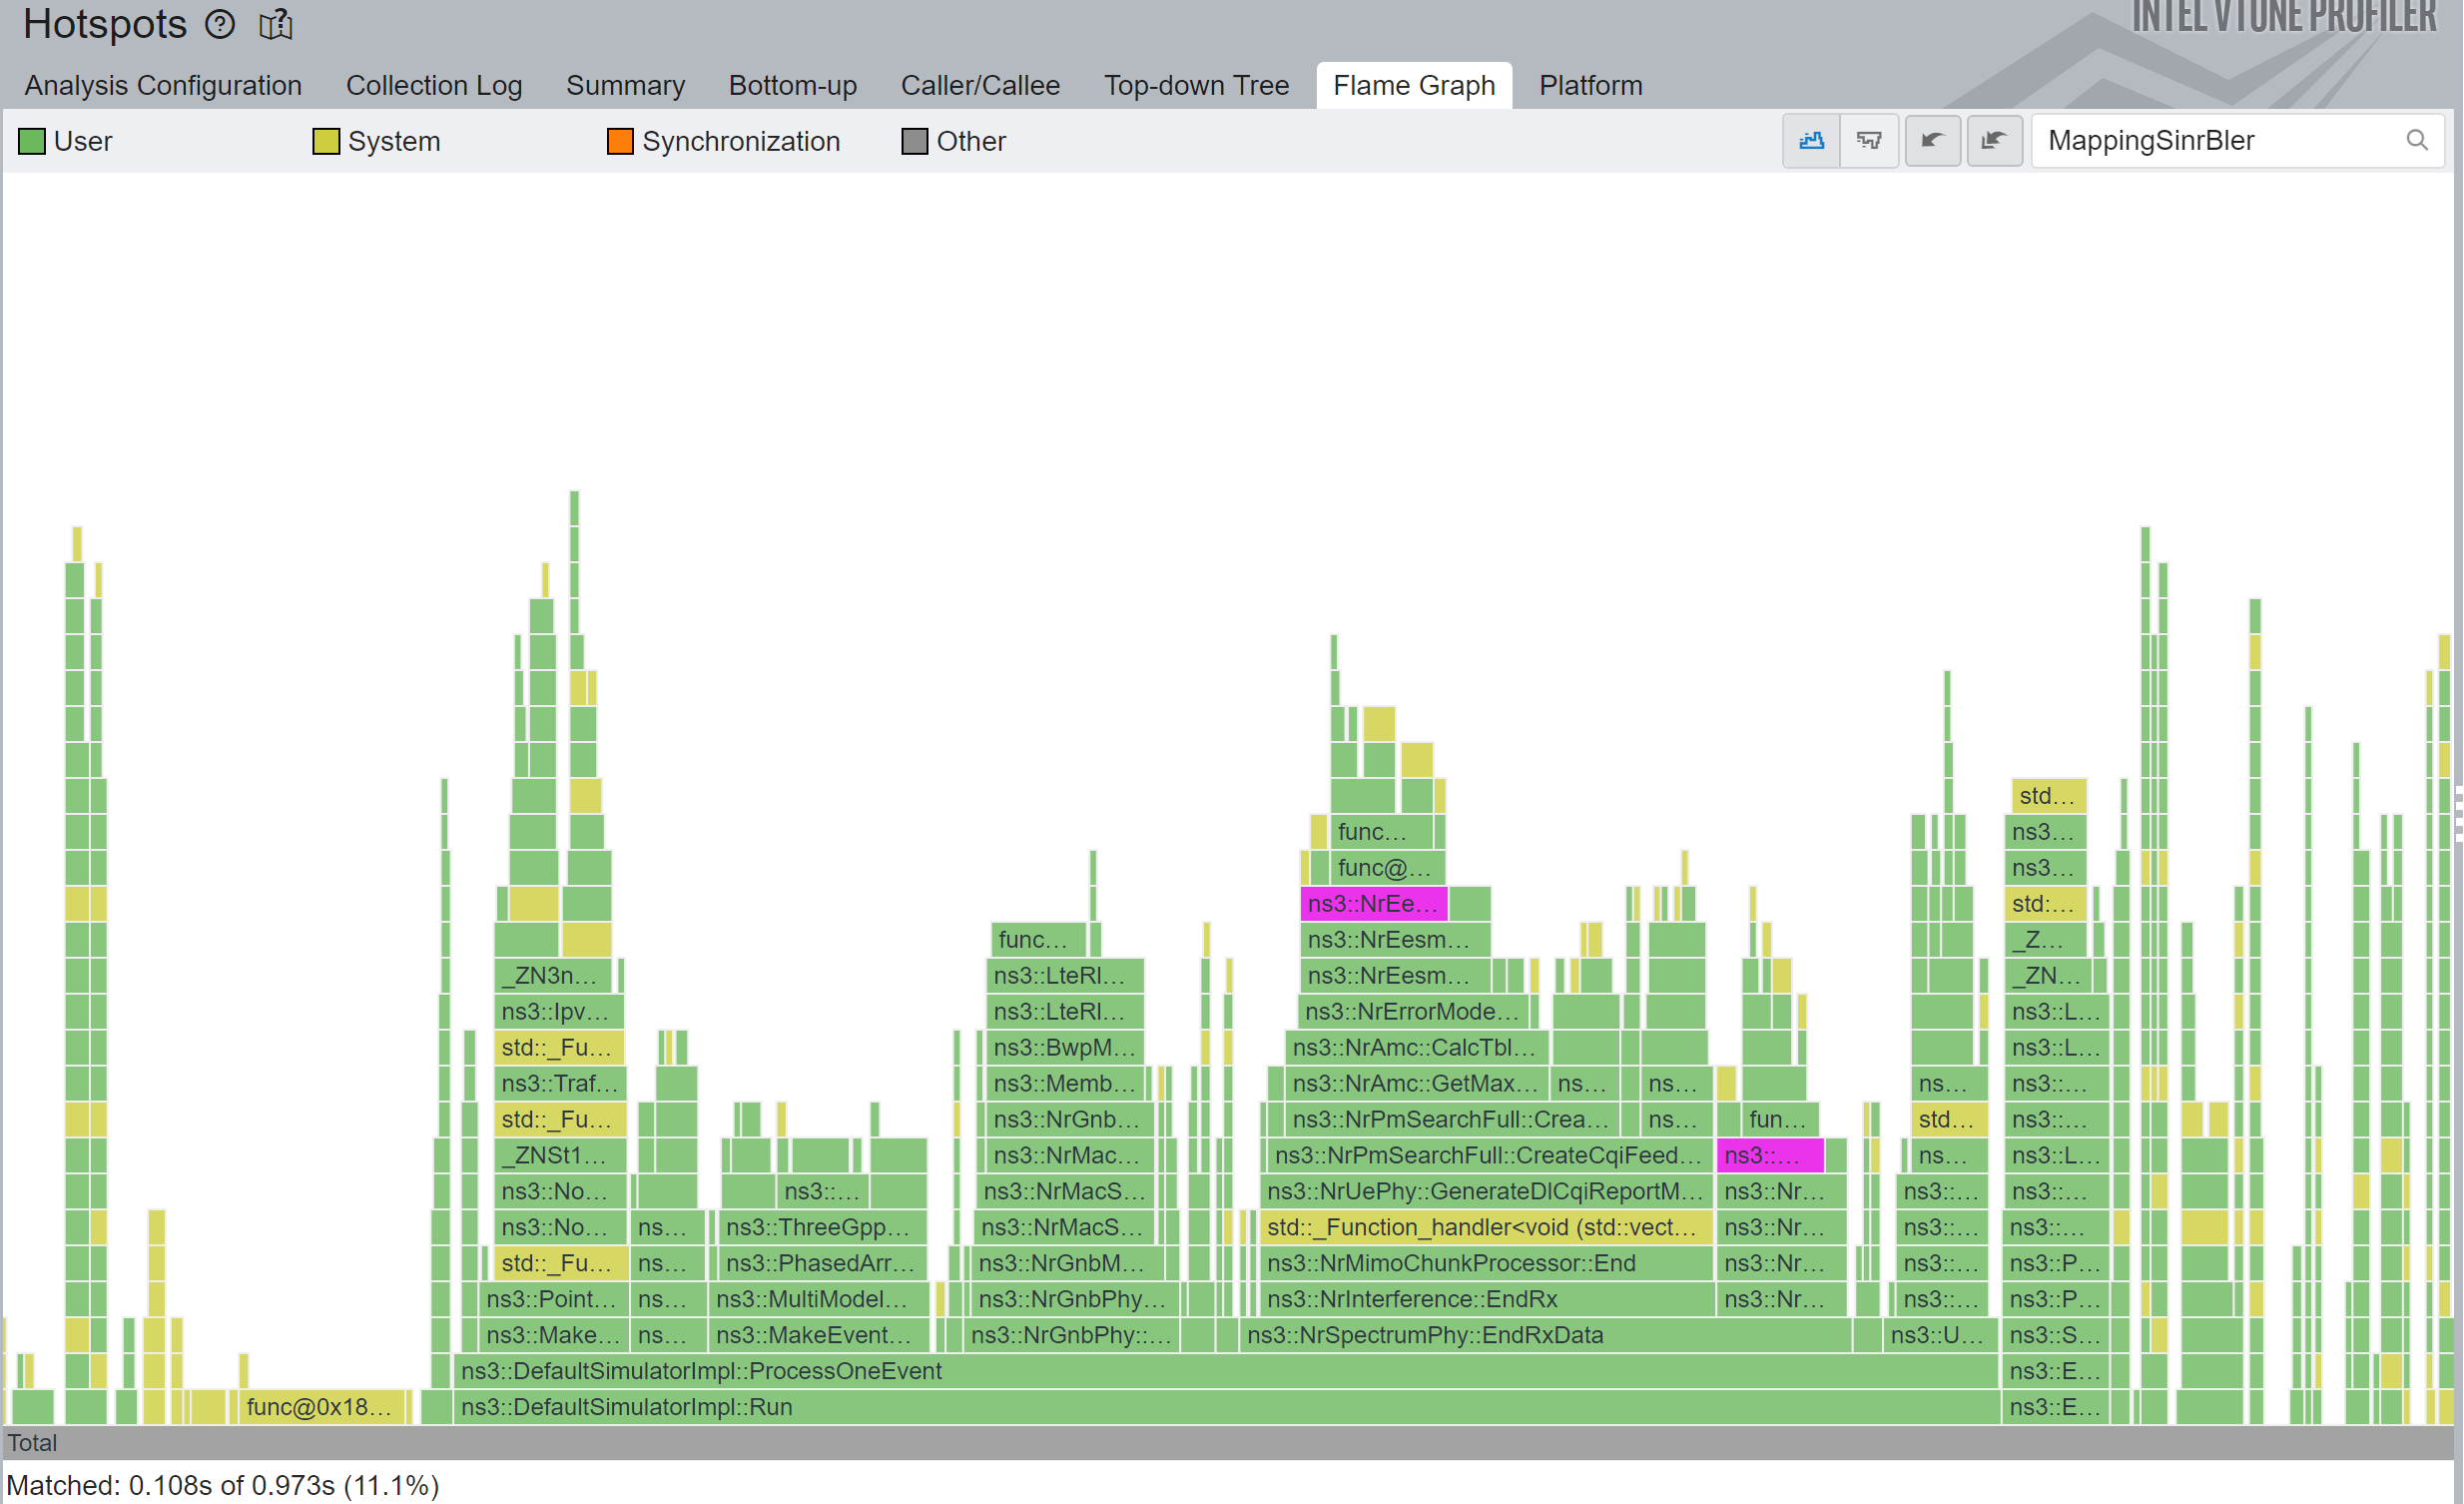
\includegraphics[width=1.0\textwidth,height=1.0\textheight]{"/assets/img/2024-03-07-the-name-is-the-speedagean/prevent-copy-before.png"}
    \caption{Before optimization}
    \label{fig:prevent-copy-before}
\end{figure}

\begin{figure}
    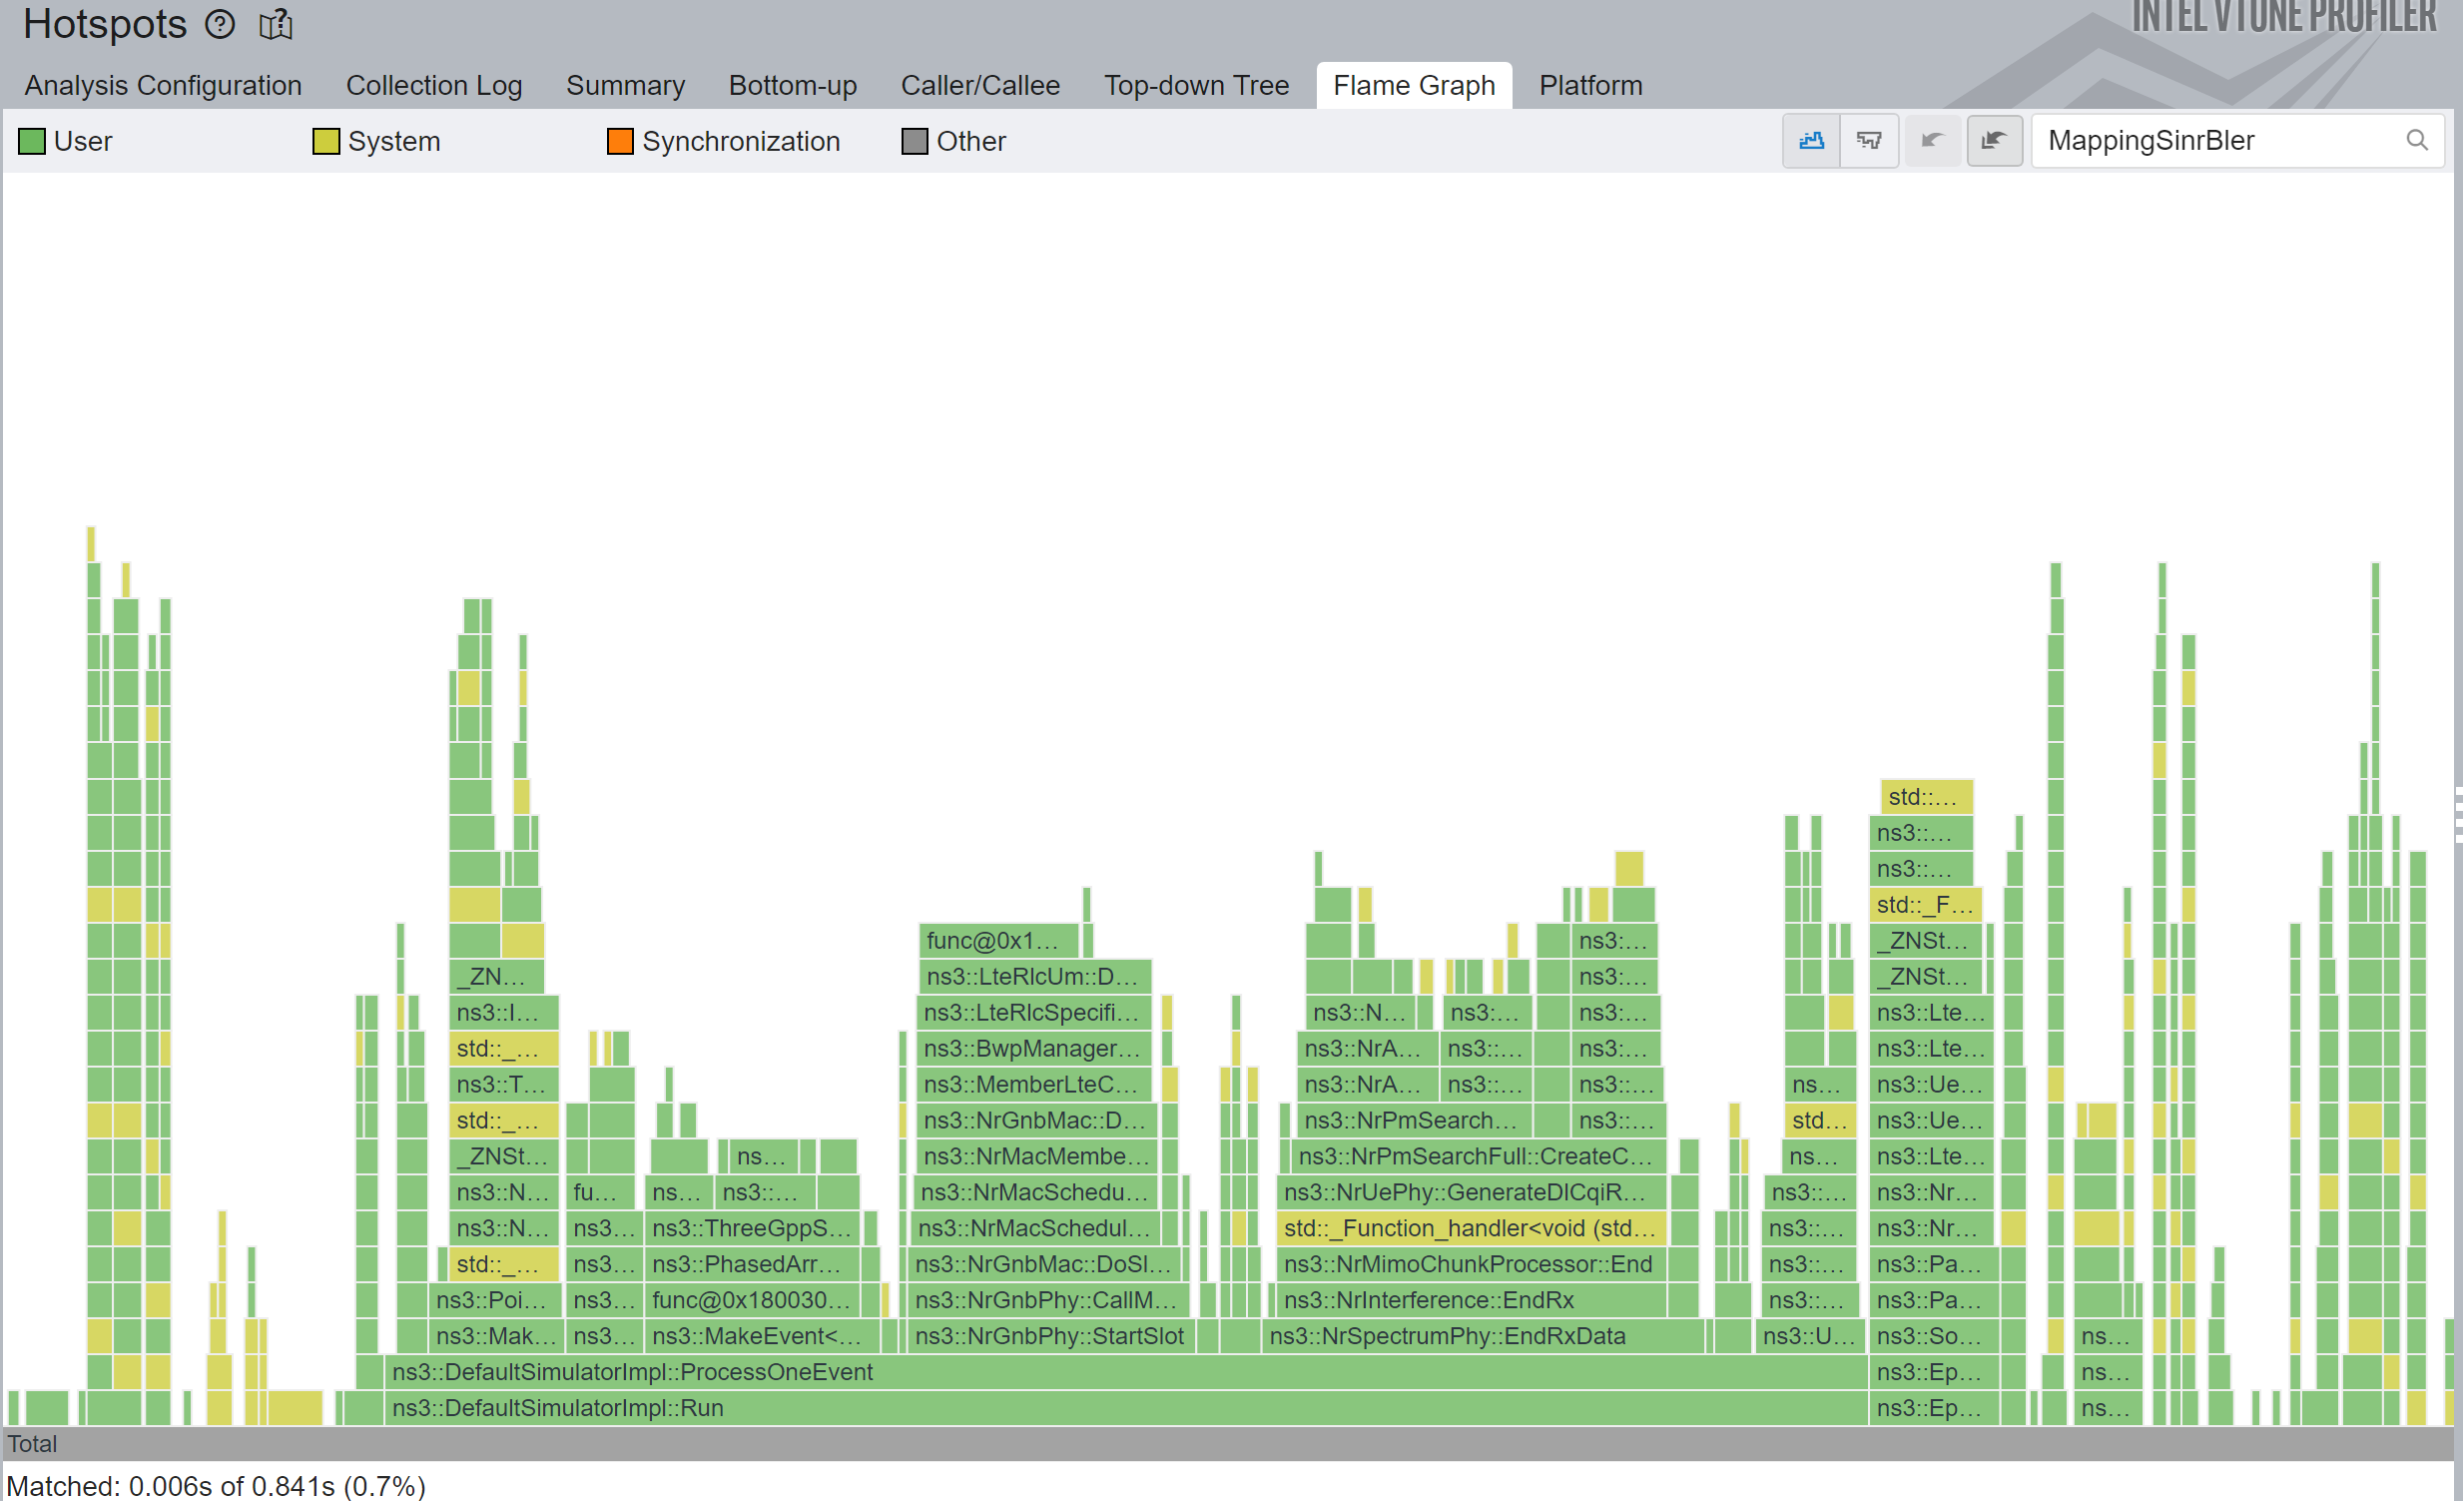
\includegraphics[width=1.0\textwidth,height=1.0\textheight]{"/assets/img/2024-03-07-the-name-is-the-speedagean/prevent-copy-after.png"}
    \caption{After optimization}
    \label{fig:prevent-copy-after}
\end{figure}

\subsection{Using the appropriate container type}

C++ offers a ton of containers that behave very similar but
are implemented very differently, which means they have different
asymptotic performance characteristics. For example eliminating
the front element in a std::vector<> has a complexity of $O(n)$, while
eliminating the front element of a std::deque<> has a complexity of $O(1)$.

Which basically means that as long as $n$ is small, they both perform
similarly, however that was not the case in the \emph{m\_txBuffer}
of LteRlcUm, currently shared by the NR module.

This is what the code looked like:

\begin{lstlisting}
void
LteRlcUm::DoNotifyTxOpportunity(LteMacSapUser::TxOpportunityParameters txOpParams)
{
    ...
    while (firstSegment && (firstSegment->GetSize() > 0) && (nextSegmentSize > 0))
    {
        NS_LOG_LOGIC("WHILE ( firstSegment && firstSegment->GetSize > 0 && nextSegmentSize > 0 )");
        NS_LOG_LOGIC("    firstSegment size = " << firstSegment->GetSize());
        NS_LOG_LOGIC("    nextSegmentSize   = " << nextSegmentSize);
        if ((firstSegment->GetSize() > nextSegmentSize) ||
            // Segment larger than 2047 octets can only be mapped to the end of the Data field
            (firstSegment->GetSize() > 2047))
        {
           ...
        }
        else // (firstSegment->GetSize () < m_nextSegmentSize) && (m_txBuffer.size () > 0)
        {
            ...
            m_txBuffer.erase(m_txBuffer.begin()); // <<<< HERE
            NS_LOG_LOGIC("        txBufferSize = " << m_txBufferSize);
        }
    }
...
}
\end{lstlisting}

By replacing the std::vector<> with a std::deque<> we got a 1.1x total
simulation speedup, or 4.8x speedup in that particular function.

\begin{figure}
    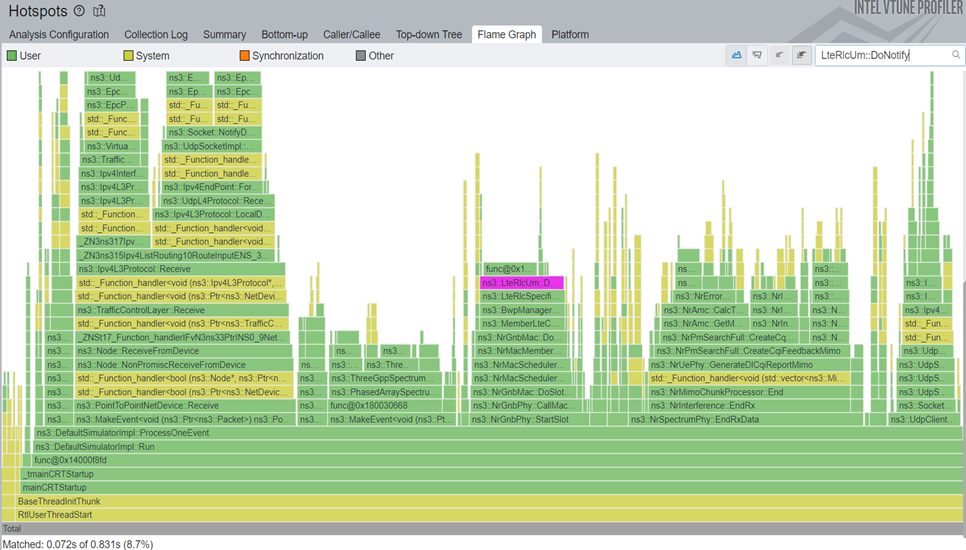
\includegraphics[width=1.0\textwidth,height=1.0\textheight]{"/assets/img/2024-03-07-the-name-is-the-speedagean/use-deque-before.png"}
    \caption{Before optimization}
    \label{fig:use-deque-before}
\end{figure}

\begin{figure}
    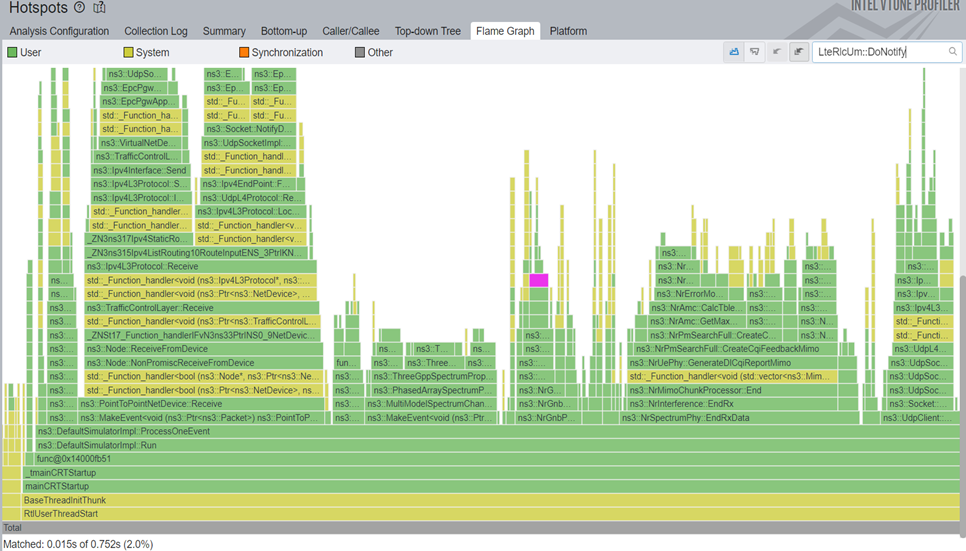
\includegraphics[width=1.0\textwidth,height=1.0\textheight]{"/assets/img/2024-03-07-the-name-is-the-speedagean/use-deque-after.png"}
    \caption{After optimization}
    \label{fig:use-deque-after}
\end{figure}

\subsection{And there is more...}

Still working on other smaller optimizations,
but nothing will ever be as significant as these ones.

Unless we go to more challenging scenarios... which we did.

\section{Absurd MIMO settings in cttc-nr-mimo-demo}

In this section, we will be using the following configuration:

\begin{itemize}
\item gNB with 2x32 antenna array, 2x8 ports, dual polarized (total of 32 ports)
\item UE with 2x8 antenna array, 2x8 ports, dual polarized (total of 32 ports)
\end{itemize}

Our client and my boss said these settings are not representative, but like
I said, I am no specialist in MIMO, so these don't have to be representative
at all for the work I am doing. Since they are so extreme, they help to point out
where the code scales badly in the new MIMO feature. And in the 2024 MWC, there
were apparently radios with 256 ports for 6G...
So we better get this scaling well to be future-proof.

These number of ports mean that our $O(n^5)$ is already in the range of $O(1024*n^3)$.
So whatever we do, we must do as cheaply as possible inside that loop.

But first, we need to perform the profiling again... And we saw the unthinkable:
the MIMO codebook search took 82\% of the total simulation time.

More on that in the next section.

\subsection{Exhaustive search can be optimal, but it is very exhausting}

In the case of MIMO codebook search, the exhaustive PMI search implemented
by NrPmSearchFull is extremely slow because the search space is very big.

I spent two weeks trying to understand how on earth MIMO works, and I got
some very superficial understanding, that was enough to identify what we
could do. My boss then said we could extract the rank and search the
wideband $i_1$ index from the channel average, and I did it. With these
two, we can skip the vast majority of the search space, and focus on finding
subband $i_2$ indices.

The full search complexity is $O(nRanks*nI1s*nSubBands*nI2s*nPortsReceiver*nPortsSender)$,
which we could say is bound by $O(n^6)$ a search space. The nI1s and nSubBands
can be extremely large numbers.

After reordering operations, we get a fast search with
$O(nPortsReceiver*nPortsSender(nSubBands+1+nI1s*nI2s+nSubBands*nI2s))$,
which is bound by a $O(n^4)$ search space.

The results are as amazing as this sounds, as can be seen in the
before \ref{fig:search-fast-before} and after \ref{fig:search-fast-after} Figures.

5x total simulation speedup, and 25x faster CreateCqiFeedbackMimo.

\begin{figure}
    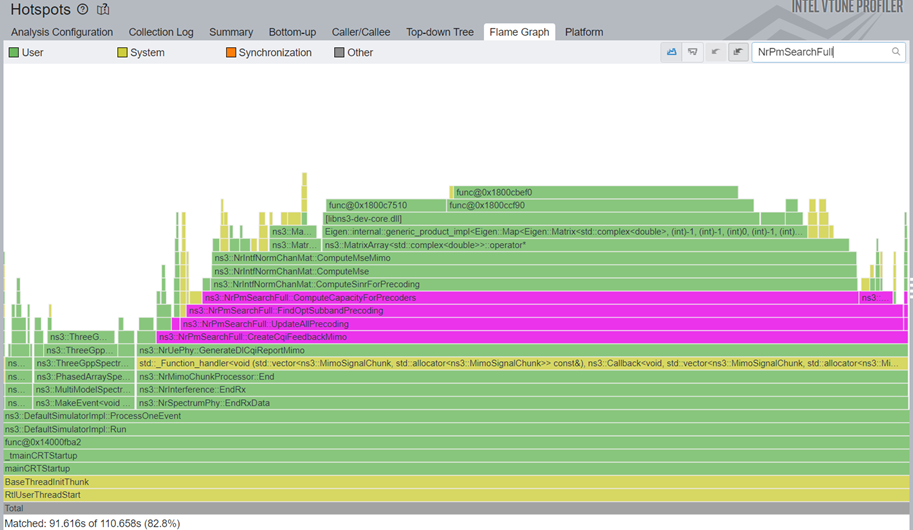
\includegraphics[width=1.0\textwidth,height=1.0\textheight]{"/assets/img/2024-03-07-the-name-is-the-speedagean/search-fast-before.png"}
    \caption{Before optimization}
    \label{fig:search-fast-before}
\end{figure}

\begin{figure}
    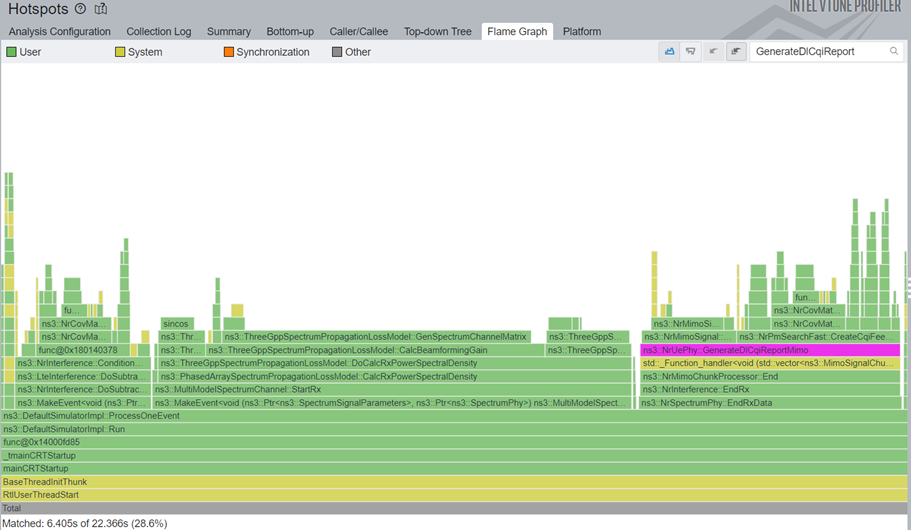
\includegraphics[width=1.0\textwidth,height=1.0\textheight]{"/assets/img/2024-03-07-the-name-is-the-speedagean/search-fast-after.png"}
    \caption{After optimization}
    \label{fig:search-fast-after}
\end{figure}

And no, we are not done yet.

\subsection{Operating on complex isn't as cheap as people would expect}

As it can be seen in the previous figures, GenSpectrumChannelMatrix is back
from the dead to torment us. It is the function contains the $O(n^5)$
archnemesis loops I mentioned at the beginning.

We took the sincos out of it, but the multiplications inside it are still
expensive. Especially since we are operating on top of complex numbers,
where each product is actually composed of 4 double multiplications plus 2 adds.

Let us have some flashbacks by looking at the loops again.

\begin{lstlisting}
while (vit != inPsd->ValuesEnd())
    {
        if ((*vit) != 0.00)
        {
            for (auto rxPortIdx = 0; rxPortIdx < numRxPorts; rxPortIdx++)
            {
                for (auto txPortIdx = 0; txPortIdx < numTxPorts; txPortIdx++)
                {
                    std::complex<double> subsbandGain(0.0, 0.0);
                    for (size_t cIndex = 0; cIndex < numCluster; cIndex++)
                    {
                        subsbandGain += directionalLongTerm(rxPortIdx, txPortIdx, cIndex) *
                                        doppler[cIndex] *
                                        channelParams->m_cachedDelaySincos(iRb, cIndex);
                    }
                    // Multiply with the square root of the input PSD so that the norm (absolute
                    // value squared) of chanSpct will be the output PSD
                    chanSpct->Elem(rxPortIdx, txPortIdx, iRb) = sqrt(*vit) * subsbandGain;
                }
            }
        }
    }
\end{lstlisting}

Notice that \emph{m\_cachedDelaySincos} and \emph{doppler} depend on cIndex,
but are completely independent on the number of ports.

But we are doing that multiplication anyways...

We can actually move all of this outside the loops, and create a temporary
array with these values.

\begin{lstlisting}
    // Compute the product between the doppler and the delay sincos
    auto delaySincosCopy = channelParams->m_cachedDelaySincos;
    for (size_t iRb = 0; iRb < inPsd->GetValuesN(); iRb++)
    {
        for (std::size_t cIndex = 0; cIndex < numCluster; cIndex++)
        {
            delaySincosCopy(iRb, cIndex) *= doppler[cIndex];
        }
    }
    ...
    while (vit != inPsd->ValuesEnd())
    {
        if ((*vit) != 0.00)
        {
            auto sqrtVit = sqrt(*vit);
            for (auto rxPortIdx = 0; rxPortIdx < numRxPorts; rxPortIdx++)
            {
                for (auto txPortIdx = 0; txPortIdx < numTxPorts; txPortIdx++)
                {
                    std::complex<double> subsbandGain(0.0, 0.0);
                    for (size_t cIndex = 0; cIndex < numCluster; cIndex++)
                    {
                        subsbandGain += directionalLongTerm(rxPortIdx, txPortIdx, cIndex) *
                                        delaySincosCopy(iRb, cIndex); // <<<< HERE
                    }
                    // Multiply with the square root of the input PSD so that the norm (absolute
                    // value squared) of chanSpct will be the output PSD
                    chanSpct->Elem(rxPortIdx, txPortIdx, iRb) = sqrtVit * subsbandGain;
                }
            }
        }
        vit++;
        iRb++;
    }
\end{lstlisting}

Yes, we did copy the sincos cache, because we can't overwrite it with doppler data,
which is updated more regularly. But we just cut the number of multiplications in half.

This patch is part of \href{https://gitlab.com/nsnam/ns-3-dev/-/merge_requests/1888}{ns-3 MR1888}.

The effects, again, are just as incredible as the sincos ones before it:
1.22x total simulation speedup, or 1.71x speedup in GenSpectrumChannelMatrix function.

Figures from before \ref{fig:precompute-delay-doppler-before} and after \ref{fig:precompute-delay-doppler-after} below show exactly the magnitude of the savings.

\begin{figure}
    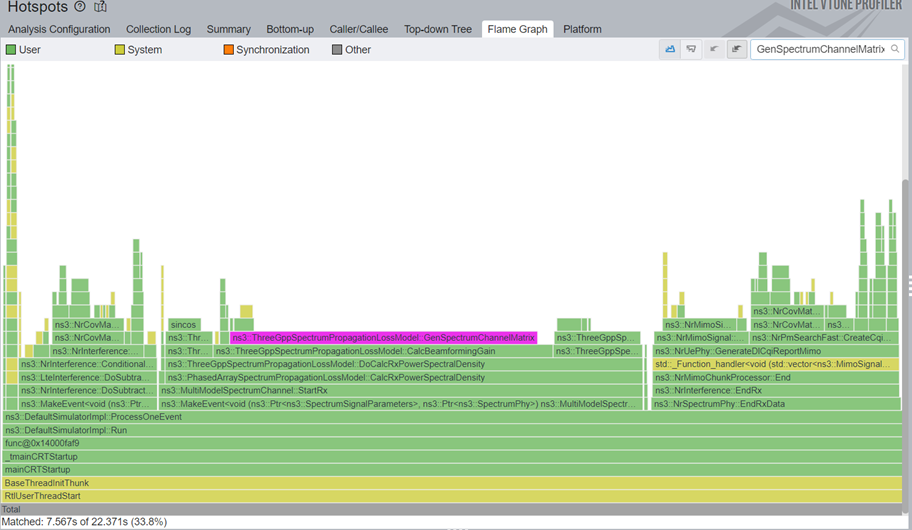
\includegraphics[width=1.0\textwidth,height=1.0\textheight]{"/assets/img/2024-03-07-the-name-is-the-speedagean/precompute-delay-doppler-before.png"}
    \caption{Before optimization}
    \label{fig:precompute-delay-doppler-before}
\end{figure}

\begin{figure}
    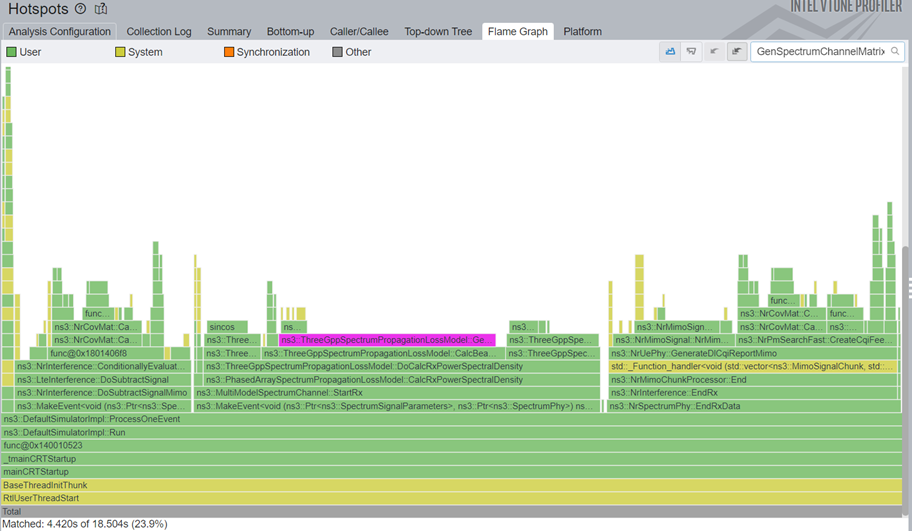
\includegraphics[width=1.0\textwidth,height=1.0\textheight]{"/assets/img/2024-03-07-the-name-is-the-speedagean/precompute-delay-doppler-after.png"}
    \caption{After optimization}
    \label{fig:precompute-delay-doppler-after}
\end{figure}

And we still have more optimization work to do before our next nr release.
When it gets released, we will make a post full of performance comparisons in the \href{https://5g-lena.cttc.es/}{5g-lena website}.

\end{document}